\documentclass{article}

\usepackage{stmaryrd}
\usepackage{amsmath}
\usepackage{amssymb}
\usepackage{amsthm}
\usepackage{relsize} 
\usepackage{bm} 
\usepackage{IEEEtrantools}
\usepackage{graphicx}
\usepackage{caption}
\usepackage{subcaption}
\usepackage{hyperref}
\usepackage{cases}
\usepackage{xfrac}
\usepackage{comment}
\usepackage{framed}
\usepackage{fancyhdr}
\usepackage{enumitem}
\usepackage{cite}
\usepackage[]{algorithm2e}
\usepackage[procnames]{listings}
\usepackage{color}
\usepackage[normalem]{ulem}

\definecolor{keywords}{RGB}{255,0,90}
\definecolor{comments}{RGB}{0,0,113}
\definecolor{red}{RGB}{160,0,0}
\definecolor{green}{RGB}{0,150,0}
 
\newcommand\pythonstyle{\lstset{language=Python, 
        basicstyle=\ttfamily\small, 
        keywordstyle=\color{keywords},
        commentstyle=\color{comments},
        stringstyle=\color{red},
        showstringspaces=false,
        identifierstyle=\color{green},
        procnamekeys={def,class}}}

\lstnewenvironment{python}[1][]
{
\pythonstyle
\lstset{#1}
}
{}

\newcommand\pythonexternal[2][]{{
\pythonstyle
\lstinputlisting[#1]{#2}}}

\oddsidemargin = 20pt
\textwidth = 420pt

\hypersetup{
     colorlinks   = true,
     linkcolor    = blue
}

\title{Project in Predictive Control and Real Time Systems}
\author{Marcus Greiff - marcusgreiff.93@hotmail.com\\ Daniel Nilsson - danielnilssonjj@gmail.com\\\\ Supervised by Fredrik Bagge Carlsson and Martina Maggio}
\begin{document}
\maketitle

\newpage
\tableofcontents
\newpage

\section{Introduction}
The control and development of small autonomous aircraft is a very interesting problem with myriad applications. In previous research, small rotorcraft have been used to build temporary rope bridges between gorges, with the mindset of eventually aiding aid fire brigades and rescue workers. Other interesting but slightly less useful examples include a quadcopters which detect the trajectories of a thrown balls to bounce it back to the tosser. When it comes to potential applications the sky is quite literally the limit.

In this project we aspire to develop new and better methods of control of the matchbox-sized crazyflie 2.0 quadcopter. The goal is to have a final product can both find and follow trajectories in space through cluttered environments, implemented in the robot operating system (ROS) and developed in Matlab/Simulink. The chief interests in the project are from the side of Bitcraze AB, developers of the crazyflie rotorcraft, who are keen to improve the control system and also to migrate to a platform using the ROS. However, if everything goes well and the final product operates as intended, Acconner AB are very interested in using it as a demo for their new short distance radar sensor, the A1 prototype, which is currently being integrated with the existing hardware at Bitcraze. The A1 sensor holds great promise in it's ability to accurately measure short distances, it's low power consumption and the possibility detection materials with different properties. For instance, the sensor can distinguish between animate tissue and a wall, potentially enabling the crazyflie to interact safely with humans. This is quite an undertaking given the four week scope of the Realtime Systems course. However, it is but the start of the project which will hopefully continue throughout the summer. As such, this report is not in it's final state, and some sections will have to be explained more thoroughly. All statements that we did not have time to support with citations, simulations and experiments have been removed in this draft.

\subsection{Goals}
With this brief background, the major goals and milestones of the can be summarised in the following seven points:
\begin{enumerate}
\item Derive and implement a discrete time model of the quadcopter dynamics, complete with system identification (written in ROS/Python/Simulink/Matlab)
\item Derive and implement and inner controller to be run on the crazyflie at high frequencies for the purpose of stabilising the rotorcraft (written in C).
\item Derive and implement and inner controller to be run on the host computer at lower frequencies to follow reference trajectory, written in (ROS/Python).
\item Investigate and implement methods of state estimation for both the inner and outer loop based on available sensors (gyroscope/accelerometer/magnetometer/pressure sensor).
\item Find and implement good ways of external motion capture if needed (written in ROS).
\item Implement an algorithm for finding a polynomial splines constituting a minimum snap trajectory through safe regions in space, and another algorithm for finding safe regions.
\item Work on the algorithms for decoding the A1-sensor data complement the control system A1-altitude measurements  (written in C).  
\end{enumerate} 

Much of these goals have already been met, and the current state of the project in relation to these goals is presented in the project summary (see \textbf{Section~\ref{sec:goalsandmilestones}}). 
\section{Dynamics}
We consider an extension of the non-linear quadcopter dynamics as derived by Lukkonen~\cite{luukkonen2011modelling}. We give a brief description of the dynamics to properly define terms which will be used in the derivation of the control scheme, but the interested reader is referred to the project repository on Github for the code and a more thorough description. Let
\begin{equation}
\boldsymbol{\xi} = \begin{bmatrix}x\\y\\z\end{bmatrix},\quad
\boldsymbol{\eta}= \begin{bmatrix}\phi\\\theta\\\psi\end{bmatrix},\quad
\boldsymbol{\omega}=\begin{bmatrix}\omega_1\\\omega_2\\\omega_3\\\omega_4\end{bmatrix},
\end{equation}
where $\boldsymbol{\xi}$ [m] denotes the position of the centre of mass in a global cartesian coordinate system, $\boldsymbol{\eta}$ [rad] is the euler-angles in the body coordinate system and $\omega_i$ [rad/s] is the angular speed of the rotor $i$. For future reference, the basis vectors in the cartesian coordinate system are written $\hat{\mathbf{\cdot}}$, and the subindexing $\mathbf{\cdot}_B$ refers to the vector of matrix defined in the body coordinate system.

The translation from the global- to the body coordinate system is done by the orthogonal rotation matrix
\begin{equation}
\mathbf{R} = 
\begin{bmatrix}
\cos(\psi)\cos(\phi) & \cos(\psi)\sin(\theta)\sin(\phi)- \sin(\psi)\cos(\phi) & \cos(\psi)\sin(\theta)\cos(\phi)+ \sin(\psi)\sin(\phi)\\
\sin(\psi)\cos(\phi) & \sin(\psi)\sin(\theta)\sin(\phi) + \cos(\psi)\cos(\phi) & \sin(\psi)\sin(\theta)\cos(\phi) - \cos(\psi)\sin(\phi)\\
 - \sin(\theta) & \cos(\theta)\sin(\phi) &  \cos(\theta)\cos(\phi)
\end{bmatrix}
\end{equation}
such that a vector defined in the body system $\mathbf{v}_B$ can be translated to the global coordinate by the mapping
\begin{equation}
\mathbf{v} = \mathbf{R}^{-1}\mathbf{v}_B = \mathbf{R}^{T}\mathbf{v}_B.
\end{equation}

The force generated by the rotor $i$ is assumed to be proportional to the rotor speed squared,
\begin{equation}
f_i = c_2 \omega_i^2 + c_1 \omega_i + c_0 \approx k_i\omega_i^2,
\end{equation}
in the positive $\hat{\mathbf{z}}_B$ direction with some constant $k_i$. In a brief system identification done by Bitcraze, a non-linear regression of measured force (or rather thrust) as a function of rotor speed yielded a quadratic relationship~\cite{antonssonRPM2015}. The approximation is deemed good enough for the purposes of the stabilising controller, but the coefficients will be identified for our hardware.

We denote the torque around each motor axis by
\begin{equation}
\tau_{M_i}\ = b\omega_i^2+I_M\dot{\omega_i}
\end{equation}
where $b$ is a drag constant and $I_M$ is the rotor inertia. By virtue of symmetry and under the assumption that $k_i\approx k \in \mathbb{R}^+\;\;\forall i$, the thrust and torque vectors in the body coordinate system can be written
\begin{equation}\label{eq:torque}
\mathbf{T}_{B} =
T \hat{\mathbf{z}}_B= 
\begin{bmatrix}
0\\
0\\
 k\sum\limits_{i = 1}^4\omega_i^2
\end{bmatrix}
, \qquad
\boldsymbol{\tau}_B = 
\begin{bmatrix}
\tau_{\phi}\\
\tau_{\theta}\\
\tau_{\psi}\\
\end{bmatrix}
=
\begin{bmatrix}
kl(-\omega_2^2 + \omega_4^2)\\
kl(-\omega_1^2 + \omega_3^2)\\
\sum\limits_{i = 1}^4\tau_{M_i}\\
\end{bmatrix}
\end{equation}
To make the model more accurate, we introduce air resistance or drag, which increases with $\dot{\boldsymbol{\xi}}$ similarly to viscous friction. This drag matrix is defined as
\begin{equation}
\mathbf{D} =
\begin{bmatrix} D_{11} & 0 & 0\\ 0 & D_{22} & 0\\ 0 & 0 & D_{33}\\\end{bmatrix}
\end{equation}
where $D_{11}=D_{22} < D_{33}$, and the coefficients remain to be estimated. With the above definitions, the non-linear dynamics of the quadcopter can then be derived from the Newton-Euler equations as
\begin{equation}
\begin{cases}
 m\ddot{\boldsymbol{\xi}} = m\mathbf{G} + \mathbf{T}_{B}-\mathbf{D}\dot{\boldsymbol{\xi}}\\
\ddot{\boldsymbol{\eta}}=\mathbf{J}^{-1}(\boldsymbol{\eta})(\boldsymbol{\tau}_B-\mathbf{C}(\boldsymbol{\eta},\dot{\boldsymbol{\eta}})\dot{\boldsymbol{\eta}}),
\end{cases}
\end{equation}
A brief description of $\mathbf{J}$ and $\mathbf{C}$ matrices can be found in \textbf{Section~\ref{sec:appendix}}, but the interested reader is referred to~\cite{luukkonen2011modelling} for a more thorough derivation of the Newton-Lagrange equations. In the work of Lukkonen, this system was simulated in continuous time, and here we will take an alternate approach in order to implement the dynamics as a discrete time ROS node in Python.

\subsection{Non-linear model}
By defining the states and control signals as

\begin{equation}
\mathbf{x} = 
\begin{bmatrix}
\boldsymbol{\xi} \\ 
\dot{\boldsymbol{\xi}} \\ 
\boldsymbol{\eta} \\ 
\dot{\boldsymbol{\eta}}
\end{bmatrix}
\in\mathbb{R}^{12\times 1}, \quad\text{and}\quad
\mathbf{u} = 
\begin{bmatrix}
T\\
\tau_{\phi}\\
\tau_{\theta}\\
\tau_{\psi}
\end{bmatrix}\in\mathbb{R}^{4\times 1}
\end{equation}
respectively, the full non-linear system can then be written
\begin{flalign}\label{eq:contsys}
\begin{split}
\dot{\mathbf{x}}(t) =&\mathbf{A}_c\mathbf{x}(t)+\mathbf{B}_c\mathbf{u}(t)+\mathbf{G}_c\\
\mathbf{y}(t) =& \mathbf{C}_c\mathbf{x}(t)
\end{split}
\end{flalign}
with 
\begin{equation}\label{eq:continuoussys}
\mathbf{A}_c=\begin{bmatrix}
\mathbf{0} & \mathbb{I}_{3\times 3} & \mathbf{0} & \mathbf{0} \\
\mathbf{0} & -\frac{1}{m}\mathbf{D} & \mathbf{0} & \mathbf{0} \\
\mathbf{0} & \mathbf{0} & \mathbf{0} &\mathbb{I}_{3\times 3} & \\
\mathbf{0} & \mathbf{0} & \mathbf{0} &-\mathbf{J}^{-1}(\boldsymbol{\eta})\mathbf{C}(\boldsymbol{\eta},\dot{\boldsymbol{\eta}}) 
\end{bmatrix},
\mathbf{B}_c=\begin{bmatrix}
\mathbf{0} &\mathbf{0}\\
\frac{1}{m}\mathbf{R}\hat{\mathbf{z}} & \mathbf{0}\\
\mathbf{0} &\mathbf{0}\\
\mathbf{0} & \mathbf{J}(\boldsymbol{\eta})^{-1}\\
\end{bmatrix},
\mathbf{G}_c\begin{bmatrix}
\mathbf{0}\\
\mathbf{G}\\
\mathbf{0}\\
\mathbf{0}\\
\end{bmatrix},
\mathbf{C}_c=\begin{bmatrix}
 \mathbf{0}_{7\times 2} & \mathbb{I}_{7\times7} & \mathbf{0}_{7\times 2}
\end{bmatrix}
\end{equation}
The $\mathbf{C}_c$ matrix was chosen to reflect the available sensory information. The height $z$ is measured by a pressure sensor, the angles $\boldsymbol{\eta}$ are retrieved from a gyroscope aboard the quadcopter and the velocities $\dot{\boldsymbol{\xi}}$ are integrated from readings of the combined sensory feedback from the accelerometer and magnetometer. In order to simulate the dynamics, the continuous time system~\eqref{eq:contsys} was implemented in Simulink (see \texttt{quadcopter\_model.m}, \textbf{Section~\ref{sec:appendix}}), and validated by comparison to the results in~\cite{luukkonen2011modelling}.

The motors in the physical process are incredibly responsive, going from $||{\boldsymbol\omega}||_{\infty} \approx 0$ to $||{\boldsymbol\omega}||_{\infty} \approx 2.5\cdot 10^4$ in $< 180$ [ms]~\cite{\cite{antonssonRPM2015}}. We have access to RPM measurements and can therefore construct a very fast PID loop for each motor to keep $\boldsymbol\omega^2$ at a desired value. Consequently, it could be an idea to investigate methods of control when using rotor speeds as control signals. If we make the assumption that the PID loops are very fast, and that the copter will be operating close to a hovering position with bounds on the control signals, it might be feasible to assume a 1:1 relashionship between desired rotor speed and actual rotor speed and not include the PID dynamics in the system matrix. The main reason for this is that including the 12 additional states will make the problem too big to solve efficiently with the MPC formulation. To accomplish this, we define a mapping from rotor speeds to thrust and torques,
\begin{equation}\label{eq:tomegamapping}
\begin{bmatrix}
T\\
\tau_{\phi}\\
\tau_{\theta}\\
\tau_{\psi}
\end{bmatrix}
=
\mathbf{M}_{\omega}\boldsymbol\omega^2
\quad\text{where}\quad
\mathbf{M}_{\omega} = 
\begin{bmatrix}
    k&    k&   k&   k\\
    0& -kl&   0& kl\\
 -kl&    0& kl&  0\\
   -b&    b&  -b&   b\\
\end{bmatrix}
\quad\text{and}\quad
\mathbf{M}^{-1}_{\omega} = 
\begin{bmatrix}
    \frac{1}{4k}& 0 & -\frac{1}{2kl} &  \frac{1}{4b}\\
    \frac{1}{4k}& -\frac{1}{2kl} & 0 & -\frac{1}{4b}\\
    \frac{1}{4k}& 0 &  \frac{1}{2kl} &  \frac{1}{4b}\\
    \frac{1}{4k}&  \frac{1}{2kl} & 0 & -\frac{1}{4b}\\
\end{bmatrix}
\end{equation}
as derived from equation~\eqref{eq:torque}. The updated continuous system, with $\mathbf{u}(t) = \boldsymbol\omega^2(t)$ is then
\begin{flalign}\label{eq:contsys2}
\begin{split}
\dot{\mathbf{x}}(t) =&\mathbf{A}^c\mathbf{x}(t)+\mathbf{B}^c\mathbf{M}_{\omega}\mathbf{u}(t)+\mathbf{G}^c\\
\mathbf{y}(t) =& \mathbf{C}^c\mathbf{x}(t)
\end{split}
\end{flalign}

No matter which continuous system is used (linear or non-linear), the discrete time system is computed using zero-order hold at a time step $h$, with the discrete state space representation
\begin{flalign}
x(t_k + h) =& \mathbf{A}_dx(t_k) + \mathbf{B}_d\mathbf{u}(t_k) + \mathbf{G}_d\\
y(t_k) =& \mathbf{C}_dx(t_k)\\
\end{flalign}
where
\begin{equation}
\mathbf{A}^d =e^{\mathbf{A}^ch},\qquad
\mathbf{B}^d =\int_0^he^{\mathbf{A}^ch} dsB^c,\qquad
\mathbf{G}^d =h\mathbf{G}^c,\qquad
\mathbf{C}^d =\mathbf{C}^c.
\end{equation}
As the final implementation of the control system is to be done in ROS (Python/C++/C), a script was written do simulate the system and included in the ROS implementation (see Figure~\ref{fig:ROSPython}).

\begin{figure}[htbp]
\centering
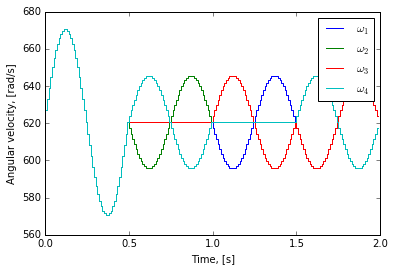
\includegraphics[width=0.5\textwidth]{figures/ROSPythonOmega.png}%
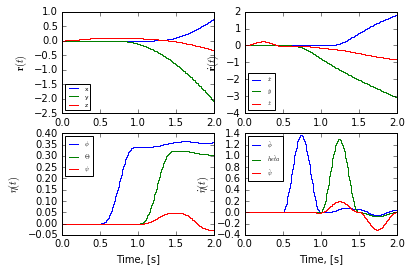
\includegraphics[width=0.5\textwidth]{figures/ROSPythonStates.png}
\rule{35em}{0.5pt}
\caption{Simulation of the discrete time quadcopter dynamics using the crazylib module implemented in ROS. \textit{Left:} Control signals in motor rotor speed similar to those used by Lukkonen to test the continuous time model. \textit{Right:} The system response with the quadcopter position and velocity in the global frame top ($\mathbf{r}$ and $\dot{\mathbf{r}}$) and the Euler angles in the body coordinate system bottom ($\boldsymbol\eta$ and $\dot{\boldsymbol\eta}$).}
\label{fig:ROSPython}
\end{figure}

The result was generated by feeding similar control signals similar to those used by~\cite{luukkonen2011modelling} to the /quadcopterModel node in ROS, and plotting the system response. Setting the same parameters as Lukkonen, the response should be very similar to the continuous time simulated response but in discrete time, which certainly is the case (compare with~\cite{luukkonen2011modelling}), thus validating the implementation of the discrete time dynamics in relation to previous work.

\subsection{Linearised dynamics}\label{sec:linearized}
Consider the continuous time system with input signal $\mathbf{u}=\boldsymbol\omega^2$, it is clear then that the non-linear part of the state-space matrices only concern the $\boldsymbol\eta,\dot{\boldsymbol\eta}$-states and the input signal. By defining the linearisation point of the euler angles around the stable point $\boldsymbol\eta_{p}=\dot{\boldsymbol\eta}_{p}=0$, and the rotor velocities around the rotor speed required to hover $\boldsymbol\omega_{p} = \sqrt{\frac{gm}{4k}}[1,1,1,1]^T$, such that the deviation from the linearisation points become
\begin{flalign}
\begin{split}
\Delta\boldsymbol\eta =& \boldsymbol\eta - \boldsymbol\eta_{p}\\
\Delta\dot{\boldsymbol\eta} =& \dot{\boldsymbol\eta} - \dot{\boldsymbol\eta}_{p}\\
\Delta\boldsymbol\omega =& \boldsymbol\omega - \boldsymbol\omega_{p}
\end{split}
\end{flalign}
Close to this point, the non-linear component of the $\mathbf{A}_c$-matrix $(\mathbf{J}^{-1}\mathbf{C}\dot{\boldsymbol\eta})$ can be linearised as
\begin{equation}
\frac{\partial\mathbf{J}^{-1}(\boldsymbol\eta)\mathbf{C}(\boldsymbol\eta,\dot{\boldsymbol\eta})\dot{\boldsymbol\eta}}{\partial \boldsymbol\eta}\Big|_{\boldsymbol\eta_p,\dot{\boldsymbol\eta}_p}= \mathbf{0}_{3\times 3},\quad\text{and}\quad
\frac{\partial\mathbf{J}^{-1}(\boldsymbol\eta)\mathbf{C}(\boldsymbol\eta,\dot{\boldsymbol\eta})\dot{\boldsymbol\eta}}{\partial \dot{\boldsymbol\eta}}\Big|_{\boldsymbol\eta_p,\dot{\boldsymbol\eta}_p}= \mathbf{0}_{3\times 3}
\end{equation}
implying that the linearized continuous-time system matrix is
\begin{equation}
\tilde{\mathbf{A}}_{\Delta\omega}=\begin{bmatrix}
\mathbf{0} & \mathbb{I}_{3\times 3} & \mathbf{0} & \mathbf{0} \\
\mathbf{0} & -\frac{1}{m}\mathbf{D} & \mathbf{0} & \mathbf{0} \\
\mathbf{0} & \mathbf{0} & \mathbf{0} &\mathbb{I}_{3\times 3} & \\
\mathbf{0} & \mathbf{0} & \mathbf{0} &\mathbf{0}
\end{bmatrix}.
\end{equation}
Using the fact that
\begin{equation}
\mathbf{J}^{-1}(\mathbf{0})=
\begin{bmatrix}
\frac{1}{I_{xx}} & 0 & 0\\
0 & \frac{1}{I_{yy}} & 0\\
0 & 0 & \frac{1}{I_{zz}}\\
\end{bmatrix}, \quad
\mathbf{R}(\mathbf{0})\hat{\mathbf{z}}_B=\hat{\mathbf{z}}=
\begin{bmatrix}
0\\
0\\
1\\
\end{bmatrix}
\end{equation}
we conclude that the linearized continuous-time $\mathbf{B}$-matrix can be written
\begin{equation}
\tilde{\mathbf{B}}_{\Delta\omega}=\frac{\partial \mathbf{B}^c(\boldsymbol\eta)\mathbf{M}_{\omega}\boldsymbol\omega^2}{\partial \boldsymbol\omega}\Big|_{\boldsymbol\eta=\mathbf{0},\boldsymbol\omega=\boldsymbol\omega_p} = \sqrt{\frac{gm}{k}}
\begin{bmatrix}
0&0&0&0\\
0&0&0&0\\
0&0&0&0\\
0&0&0&0\\
0&0&0&0\\
k&k&k&k\\
0&0&0&0\\
0&0&0&0\\
0&0&0&0\\
0 & \frac{-kl}{I_{xx}} & 0 & \frac{kl}{I_{xx}}\\
\frac{-kl}{I_{yy}} & 0 & \frac{kl}{I_{yy}} & 0\\
\frac{-b}{I_{zz}} & \frac{b}{I_{zz}} & \frac{-b}{I_{zz}} & \frac{b}{I_{zz}} \\
\end{bmatrix}
\end{equation}
It is then clear that using this linearised process model
\begin{flalign}\label{eq:linprocess}
\begin{split}
\dot{\Delta\mathbf{x}} &= \tilde{\mathbf{A}}_{\Delta\omega}\Delta\mathbf{x} + \tilde{\mathbf{B}}_{\Delta\omega}\Delta\boldsymbol\omega\\
\Delta\mathbf{y} &= \mathbf{C}_c\Delta\mathbf{x}
\end{split}
\end{flalign}
the number of observable and controllable states are
\begin{equation}
\begin{cases}
\text{rank}\Big(\begin{bmatrix}  \tilde{\mathbf{B}}_{\Delta\omega}& \cdots &\tilde{\mathbf{A}}_{\Delta\omega}^{n-1}\tilde{\mathbf{B}}_{\Delta\omega}\end{bmatrix}\Big) = 8 \neq 12\\
\text{rank}\Big(\begin{bmatrix} \mathbf{C}_c^T& \cdots &(\mathbf{C}_c\tilde{\mathbf{A}}_{\Delta\omega}^{n-1})^T\end{bmatrix}^T\Big) = 8 \neq 12
\end{cases}
\end{equation}
respectively. Closer investigation shows that we have a pole-zero cancellation of the positional $x,y$-states and their derivarives, implying that we need to have external motion capture of these states in order to use Kalman filters for state estimation (requiring full observability) or linear quadratic gaussian regulator for reference tracking (requiring full controllability). This could in theory be done by integrating measurements from the accelerometer twice and introducing a complementary filter to decrease positional drift in stationarity, but the approach is infeasible in reality and a better option is to use external of motion capture.

\subsection{Inner stabilising controller}\label{sec:PD}
The system is inherently unstable as the only truly stable position is when the copter hovers at a certain point in space, i.e. $\dot{\boldsymbol\xi}=\boldsymbol\eta=\dot{\boldsymbol\eta}=0$. In addition, we know that the x- and y-positions are unobservable and uncontrollable (as shown in \textbf{Section~\ref{sec:linearized}}), meaning the we cannot have any sort of positional control using designs based solely on ~\eqref{eq:contsys}. However, the elevation is observable and before we tackle positional control, system stability needs to be established. This stabilising controller can be run on the crazyflie at very high frequencies (currently, the loop on the crazyflie is run at 500 Hz) and could if written correctly increase overall performance of the final implementation. In this section, we define three such controllers controllers with the control signal 
\begin{equation}
\mathbf{u} = 
\begin{bmatrix}
z_{ref}&
\phi_{ref}&
\theta_{ref}&
\psi_{ref}&
\dot{z}_{ref}&
\dot{\phi}_{ref}&
\dot{\theta}_{ref}&
\dot{\psi}_{ref}&
\end{bmatrix}^T\in\mathbb{R}^{8\times 1},
\end{equation}
with subindices $(\cdot)_{ref}$ denotes reference values for the respective state.

A common way of accomplishing the goal is by using a non-model based design, and implementing a PD-controller. Such a controller was derived in e.g.~\cite{luukkonen2011modelling}~\cite{dikmen2009attitude}, and can be summarised in the scheme
\begin{flalign}
\begin{split}
T=&(g + K_{D,z}(\dot{z}_{ref} - \dot{z})) + K_{P,z}(z_{ref} - z))\frac{m}{\cos(\phi)\cos(\theta)}\\
\tau_{\phi}=&(K_{D,\phi}(\dot{\phi}_{ref} - \dot{\phi})) + K_{P,\phi}(\phi_{ref} - \phi))I_{xx}\\
\tau_{\theta}=&(K_{D,\theta}(\dot{\theta}_{ref} - \dot{\theta})) + K_{P,\theta}(\theta_{ref} - \theta))I_{yy}\\
\tau_{\psi}=&(K_{D,\psi}(\dot{\psi}_{ref} - \dot{\psi})) + K_{P,\psi}(\psi_{ref} - \psi))I_{zz}
\end{split}
\end{flalign}
In using this controller, setting all references to 0 results in a stable hovering system (in the eight controllable states) assuming the state estimation is good. In our implementations, we also include the mapping of thrusts and torques to references in rotor speeds, given by~\eqref{eq:tomegamapping}. Note that the controller is non-linear in terms of thrust, and using the PD augmented system for model based outer loop control (such as MPC) does not capture the full PD controller dynamics.

As an alternative, a fully linear LQR-controller is proposed for the same purpose, using the linearised model~\eqref{eq:linprocess} and only including the controllable modes of~\eqref{eq:contsys}. By the standard approach presented in~\cite{glad2000control}, the cost function is defined as
\begin{equation}
J = \int_0^{\infty} \mathbf{x}^T(t)\mathbf{Q}\mathbf{x}(t) + \mathbf{u}^T(t)\mathbf{R}\mathbf{u}(t)dt
\end{equation}
where $\mathbf{Q},\mathbf{R} > \mathbf{0}$ determines the costs of certain states and control signals respectively. The  optimal linear feedback law is then
\begin{equation}
\mathbf{u}= -\underbrace{\mathbf{R}^{-1}\mathbf{B}^T\mathbf{S} }_{\mathbf{K}}\mathbf{x}
\end{equation}
where the symmetric matrix $\mathbf{S}$ solves the associated Riccati equation,
\begin{equation}
\mathbf{A}^T\mathbf{S}+\mathbf{S}\mathbf{A}-\mathbf{S}\mathbf{B}\mathbf{R}^{-1}\mathbf{B}^T\mathbf{S}+\mathbf{Q}=0.
\end{equation}
This method naturally has the drawback of using the linearised model, which only accurately describes the system close to the stable, hovering state. But by bounding the pitch and yaw angles to $\phi,\theta \in [-0.5,0.5]$ rad, the controller performs very well. One inherent disadvantage with LQR is that it is fundamentally a proportional state feedback controller. A a consequence, it may give rise to stationary errors. To combat this issue, an LQR scheme with integrator (LQRi) was implemented by introducing four additional states,
\begin{equation}
\mathbf{x}_i = \begin{bmatrix} z_i&\phi_i & \theta_i & \psi_i�\end{bmatrix}^T \in \mathbb{R}^{4\times 1}
\end{equation}
such that
\begin{equation}
\mathbf{x}_i = \int\mathbf{e}(t) dt = \int\mathbf{C}\mathbf{x} - \mathbf{y} dt,\qquad\text{with} \;\;\mathbf{C} = \begin{bmatrix} \mathbb{I}_{4\times 4} &  \mathbf{0}_{4\times 4}\end{bmatrix}
\end{equation}
thereby only integrating the positional control errors, $\mathbf{e}(t)$. The reason for not integrating control errors in the velocity is to avoid duplicate states (which in this case renders the system uncontrollable eliminating the possibility of using an LQR scheme).

The extended state space model becomes
\begin{flalign}\label{eq:contsys}
\begin{split}
\dot{\mathbf{x}}_e(t) =&\mathbf{A}_e\mathbf{x}(t)+\mathbf{B}_e\mathbf{u}(t)+\mathbf{G}_e\\
\mathbf{y}(t) =& \mathbf{C}_e\mathbf{x}(t)
\end{split}
\end{flalign}
with the extended state vector $\mathbf{x}_e = \begin{bmatrix} \mathbf{x} & \mathbf{x}_i \end{bmatrix}^T \in \mathbb{R}^{12\times 1}$ and
\begin{align}
\begin{split} \;\;
\mathbf{A}_e = \begin{bmatrix} \mathbf{A}_c & \mathbf{0}_{8\times4} \\ \mathbf{C} & -\mathbb{I}_{4\times 4} \end{bmatrix} \in\mathbb{R}^{12\times 12}, \;\;
\mathbf{B}_e =  \begin{bmatrix} \mathbf{B}_c \\ \mathbf{0}_{4\times 4} \end{bmatrix} \in \mathbb{R}^{12\times 4}, \;\;
\mathbf{C}_e \in \mathbb{R}^{N\times 12},  \;\;
\mathbf{G}_e \in \mathbb{R}^{12\times 1}
\end{split}
\end{align}
Here, the integer $4\leq N\leq8$ denotes the number of observed states (not confined to the four positional used in $\mathbf{C}_e$, but can output velocities as well).

In order to allow large integral gains, the common conditional anti-windup (AW) scheme was implemented so as to set the integral part to zero when having any of the four of the rotor speeds in saturation. The implemented AW scheme can be summarised in terms of the positional control error,
\begin{equation}
\begin{cases}
\mathbf{e}(t) := \mathbf{C}\mathbf{x} - \mathbf{y}, \quad\text{if}\quad\text{sat}(\boldsymbol\omega) - \boldsymbol\omega = \mathbf{0}\\
\mathbf{e}(t) :=\mathbf{0}, \quad\quad\quad\;\;\;\text{if}\quad\text{sat}(\boldsymbol\omega) - \boldsymbol\omega \neq \mathbf{0}
\end{cases},
\end{equation}
with the saturation function defined as
\begin{equation}
\text{sat}(x) = \begin{cases}
x_{max} \qquad x_{max} < x\\
x \qquad\quad\; \;x_{min}\leq x \leq x_{max}\\
x_{min}\qquad x < x_{min}\end{cases}
\end{equation}
Using this effectively disablines integral action when any motor is in a saturated state, and has the added benefit of being very predictable. When setting up the state space model for use in MPC, we would in practice only have to define two different linearised state space models (the LQR when in saturation and the LQRi otherwise). The only downside is the additional four states, which greatly increase the complexity of the optimisation problem in MPC.

The three stabilising controllers were simulated using the parameters described in the work of Lukkonen~\cite{luukkonen2011modelling} (for which the above PD regulator was developed and tuned) and at an inner loop rate of 100 Hz (note that the original stabilising controller on the crazyflie runs at 500 Hz). The generated reference trajectory lowpass filtered unit steps the amplitudes $z\in[0,30]$ [m] and $\phi,\theta,\psi \in[-0.3,0.3]$  [rad], which is far more aggressive than anything that will be run on the real process (see Figure~\ref{fig:LQR-PD-comp}). The LQG regulators were tuned to give reasonable trajectory following in terms of Euler angles, with more pronunciation of yaw and elevation (as the yaw will later be assumed to be 0 in the external loop). As expected the LQG-controller performs well, but also yields the predicted steady state errors. In the depicted simulation, the stationary error were to be of magnitude 7 cm at $t\approx 37$ s, which is unacceptable precise indoor flying. As a contrast, both the PD and LQRi (with AW) yield errors of $\approx 0.1$ cm less than 10 seconds after a reference change, with the error still decreasing. We also note that the reference following in elevation is much more precise with the LQRi compared to the PD alternative, and that it is only outperformed by the PD in terms of overshoot when making large reference changes in angular positions. However, an acceptable angular error of $<0.005$ [rad] is reached around the same time with both regulators. In conclusion, the PD and LQRi perform almost en par, with a slight edge to the LQRi in terms of altitude changes and in less aggressive trajectories. Both should be implemented and tested on the physical process.
\begin{figure}[htbp]
\centering
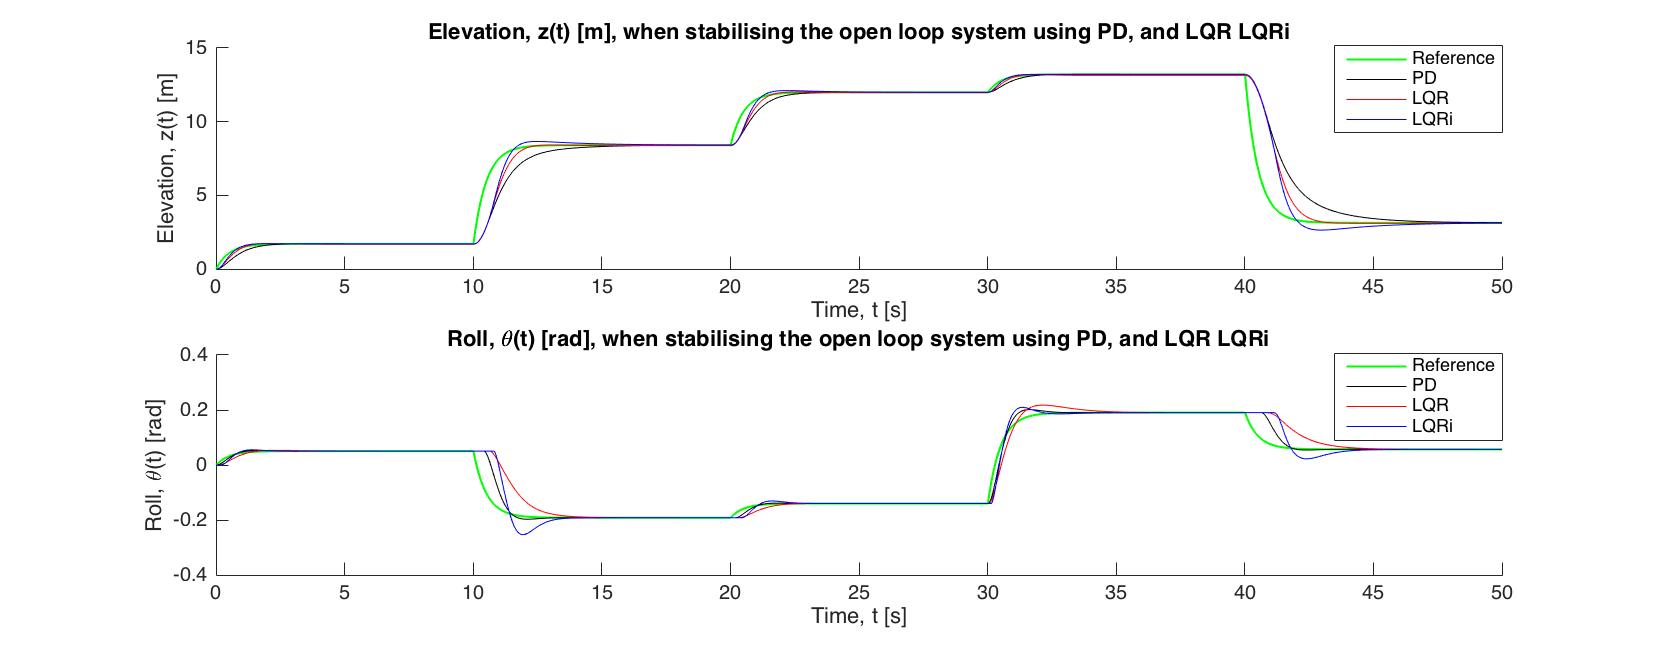
\includegraphics[width=\textwidth]{figures/innerLoopStates.png}
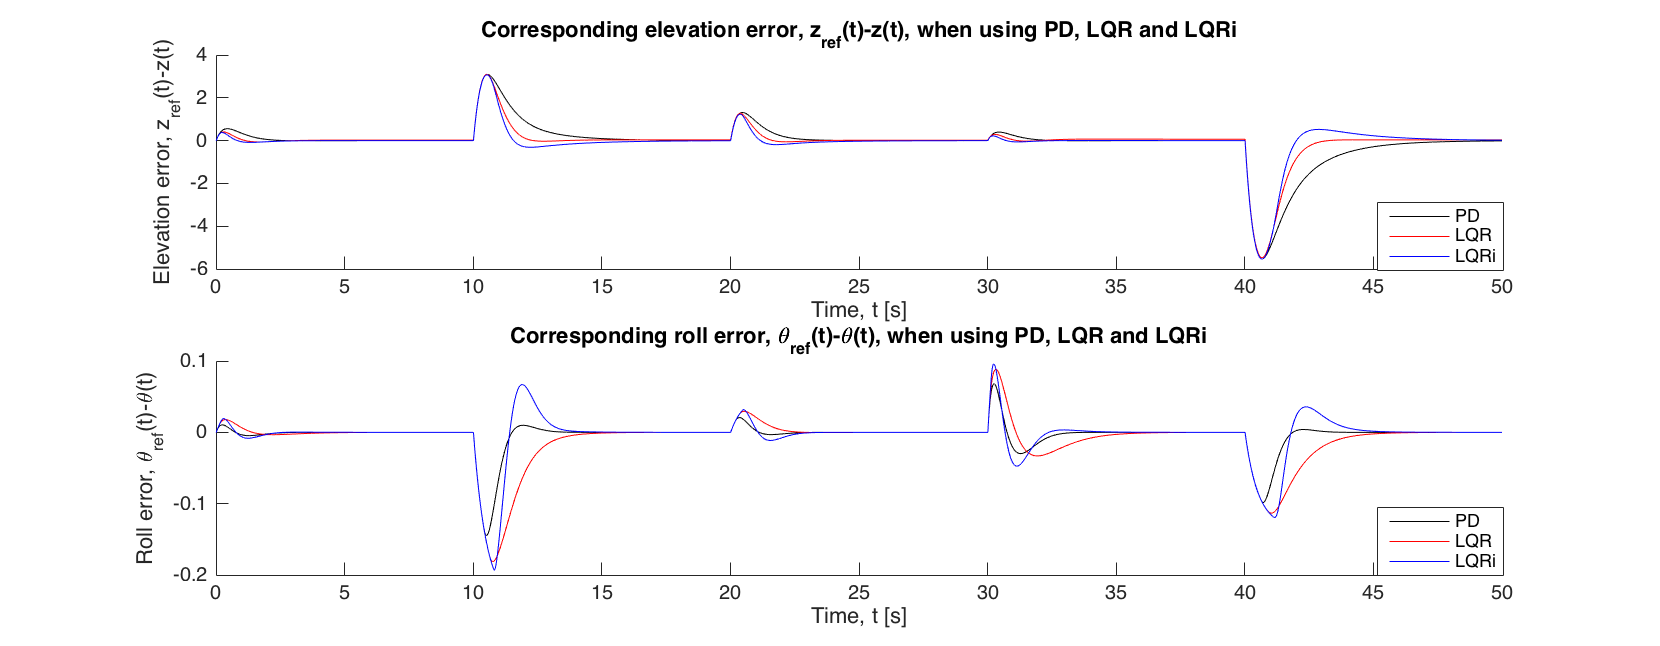
\includegraphics[width=\textwidth]{figures/innerLoopError.png}
\rule{35em}{0.5pt}
\caption{Comparision between the stabilising controllers with simulated elevation and roll (top) and the corresponding control errors (bottom).}
\label{fig:LQR-PD-comp}
\end{figure}

\clearpage\section{State estimation}
To estimate the states properly, many approaches are considered and compared in simulation before making a real time implementation. As we know from previous sections, the positions and velocities in the x- and y-directions are unobservable in the considered non-linear dynamics. Since these four states are not needed in stabilising the quadcopter, our approach will be to estimate the remaining eight states on the quadcopter and run this in conjunction with a stabilising inner controller (discussed above). This inner loop will be run at $\approx 100$ Hz and can be completely independent of external control and estimation. In order to estimate the four unobservable states, a kinect 1 camera will be run on the host computer, yielding positional measurements at $\approx 30$ Hz. These measurements will not be good enough to accurately determine the $x$- and $y$-velocities, for which the acceleration data is required. However, this data will be delayed when sent to the host computer from the crazyflie via bluetooth, and likewise, the estimated positions and speeds will suffer from a time delay when transmitted back to the crazyflie.

The problem in the inner loop is to accurately estimate the eight states
\begin{equation}
\hat{\mathbf{x}}^{(inner)}=\begin{bmatrix} z &\phi &\theta &\psi&\dot z &\dot\phi &\dot\theta &\dot\psi\end{bmatrix}^T
\end{equation}
given the torques and thrusts or the rotor angular speeds, subject to constraints in computational power and the highly non-linear dynamics of the crazyflie. To achieve this, a regular Kalman filter (KF) is tested, using the dynamics linearised around the stable hovering state to compute the filter gain ~\cite{glad2000control}. In addition the extended kalman filter (EKF) is tested. The EKF effectively linearises the system around the previous state estimate on each time step, which is done by computing an expression for the Jacobian offline and then evaluating it on-line. As the dynamics matrix contains inverses, this puts great constraints on how fast the inner loop can be run. Finally, the unscented Kalman filter (UKF) and generic particle filter (GPF) are implemented and tested on the non-linear dynamics.

Similarily, the problem in the outer loop is to accurately estimate the states
\begin{equation}
\hat{\mathbf{x}}^{(outer)}=\begin{bmatrix} x & y & z  & \dot x & \dot y & \dot z  \end{bmatrix}^T
\end{equation}
given time delayed measurements of quadcopter acceleration, current measurements of position from the kinect and predict the future position and speed of the quadcopter to combat the time delay in transmitting data back to the crazyflie. Fo this purpose a regular KF is tested along with an asynchronous Kalman filter of our own design.

\subsection{Discrete extended kalman filter (EKF)}
The regular discrete Kalman filter (KF) is omitted for brevity, but the EKF is implemented using the nonlinear system representation
\begin{flalign}\label{eq:nonlindyn}
\begin{split}
\mathbf{x}_{k+1} =& \mathbf{F}(\mathbf{x}_k,\mathbf{u}_k,\mathbf{v}_{k+1})\\
\mathbf{y}_{k} =& \mathbf{H}(\mathbf{x}_k,\mathbf{e}_{k+1})
\end{split}
\end{flalign}
denoting the respective state and measurement equation Jacobians as
\begin{equation}
\mathbf{J}^F_k = \frac{\partial \mathbf{F}(\mathbf{x}, \mathbf{u}_k, \mathbf{v})}{\partial \mathbf{x}}\Big|_{\mathbf{x}_k}
\qquad
\mathbf{J}^H_k = \frac{\partial \mathbf{H}(\mathbf{x}, \mathbf{e})}{\partial \mathbf{x}}\Big|_{\mathbf{x}_k}
\end{equation}
assuming a measurement noise zeros mean gaussian noise, with
\begin{equation}\label{eq:measnoise}
\mathbf{v}_{k} \sim\mathcal{N}(0,\mathbf{Q})\quad\mathbf{e}_{k} \sim\mathcal{N}(0,\mathbf{R}).
\end{equation}

Commonly used in GPS systems, the EKF is situational and not an optimal filter as the Jacobians used in the covariance prediction is a first order approximation in a multivariate taylor series expansion. As such, we only get an estimated covariance and not the true covariance, which may cause the state estimation to diverge if the system is non-linear enough and enough time passes. If the system, like the quadcopter process, is badly conditioned and we force it to great extremes (i.e. flying aggressivly) the EKF may fail. For a more thorough theoretical discussion on the EKF, the reader is referred to~\cite{terejanu2008extended}. 

In our implementation, the Jacobian $\mathbf{J}^F_k$ is computed offline and stored as a symbolic expression to be evaluated on each iteration (see Algortithm~\ref{fig:algEKF}). The initial covariance and  Expressing the Jacobian to a non-linear system including inverses (recall $\mathbf{J}^{-1}$ in equation~\eqref{eq:continuoussys}) could put constraints on the rate at which the estimations are made, as evaluation of the expression may take considerable time.

\begin{center}
\begin{minipage}{.6\linewidth}
\begin{algorithm}[H]
 Initialize: $\mathbf{x}_0$, $\mathbf{P}_0$, $\mathbf{Q}$, $\mathbf{R}$, $\mathbf{F}(\mathbf{x},\mathbf{u})$, $\mathbf{C}_d$, $\mathbf{J}^F(\mathbf{x})$\;
 \BlankLine
 \For{k = 1,...,$k_{max}$}{
 \BlankLine
 Receive $\mathbf{u}_k, \mathbf{z}_k$\;
 \BlankLine
 \textit{Prediction step}\\
 $\hat{\mathbf{x}}_{k}^- = \mathbf{F}(\hat{\mathbf{x}}_{k-1},\mathbf{u}_{k-1}, \mathbf{v})$\;
 $\mathbf{P}_{k}^-= \mathbf{J}^F_{k-1}\mathbf{P}_{k-1} \mathbf{J}^F_{k-1} + \mathbf{Q}$\;
 \BlankLine
 \textit{Correction step}\\
 $\mathbf{K}_{k} = \mathbf{P}_{k}^-\mathbf{C}_d^T(\mathbf{C}_d \mathbf{P}_{k}^-\mathbf{C}_d^T + \mathbf{R})^{-1}$\;
 $\hat{\mathbf{x}}_{k} = \hat{\mathbf{x}}_{k}^- + \mathbf{K}_k(\mathbf{y_k} -\mathbf{C}_d\mathbf{x}^-_k)$\;
 $\mathbf{P}_k = (\mathbb{I} - \mathbf{K}_k\mathbf{C}_d)\mathbf{P}_{k}^-$\;
 }
 \BlankLine
\caption{Rough outline of the discrete time extended Kalman filter (EKF)}
\label{fig:algEKF}
\end{algorithm}
\end{minipage}
\end{center}
For the considered dynamics, the measurement function $\mathbf{H(x,e)}$ is linear and can therefore be replaced by the discrete time measurement matrix in  ~\eqref{eq:continuoussys}, such that $\mathbf{H(x,e)} = \mathbf{C}_d\mathbf{x}$, with $\mathbf{J}^H_k = \mathbf{C}_d\forall\mathbf{x}$.

\subsection{Unscented kalman filter (UKF)}
The unscented Kalman filter is well described in~\cite{wan2000unscented}, where it is qualitatively compared to the EKF on the chaotic Mackey Glass time series. The interested reader is referred to~\cite{wan2000unscented} for more details, but a rough sketch of the algorithm as implemented in Python/ROS/Simulink is given (see Algorithm~\ref{fig:algUKF}) with a few cliff notes. For consistency, the UKF uses the same system description and assumptions defined in the previous section on the EKF, see equations~\eqref{eq:nonlindyn} to~\eqref{eq:measnoise}.

\begin{center}
\begin{minipage}{.6\linewidth}
\begin{algorithm}[H]
 Initialize: $\mathbf{x}_0$, $\mathbf{P}_0$, $W^m$, $W^c$, $\mathbf{Q}$, $\mathbf{R}$, $\mathbf{F}(\mathbf{x},\mathbf{u})$, $\mathbf{H}(\mathbf{x})$\;
 \BlankLine
 \For{k = 1,...,$k_{max}$}{
 \BlankLine
 Receive $\mathbf{u}_{k-1}, \mathbf{z}_k$\;
 \BlankLine
 \textit{Compute weights and $\sigma$-points}\\
 $\sqrt{\mathbf{P}} = \sqrt{L + \lambda}\cdot cholesky(\mathbf{P}_{k-1})^T$\;
 $X_{\sigma} = [\mathbf{x}_{k-1}, \mathbf{x}_{k-1} - \sqrt{\mathbf{P}}, \mathbf{x}_{k-1} + \sqrt{\mathbf{P}}]$\;
 \BlankLine
 \textit{Prediction step}\\
 \For{i = 1,...,2L+1}{
 $X^{f}_{i} = \mathbf{F}(X_{\sigma,i},\mathbf{u}_{k-1}, \mathbf{v}_k)$\;
 $Y^{f}_{i} = \mathbf{H}(X_{f,i}, \mathbf{e}_k)$\;
 }
 $\hat{\mathbf{x}}_k^- = \sum\limits_{i = 1}^{2L+1}W^m_iX^f_{i}$\;
 $\hat{\mathbf{y}}_k^- = \sum\limits_{i = 1}^{2L+1}W^m_iY^f_{i}$\;
 $\mathbf{P}_{xx} = \sum\limits_{i = 1}^{2L+1}W^c_i(\hat{\mathbf{x}}_k^- -X^f_{i})(\hat{\mathbf{x}}_k^- -X^f_{i})^T$\;
 $\mathbf{P}_{xy} = \sum\limits_{i = 1}^{2L+1}W^c_i(\hat{\mathbf{x}}_k^- -X^f_{i})(\hat{\mathbf{y}}_k^- -Y^f_{i})^T$\;
 $\mathbf{P}_{yy} = \sum\limits_{i = 1}^{2L+1}W^c_i(\hat{\mathbf{y}}_k^- -Y^f_{i})(\hat{\mathbf{y}}_k^- -Y^f_{i})^T$ \;
 \BlankLine
 \textit{Correction step}\\
 $\mathbf{K}_{k} = \mathbf{P}_{xy}\mathbf{P}_{yy}^{-1}$\;
 $\hat{\mathbf{x}}_{k} = \hat{\mathbf{x}}_{k}^- + \mathbf{K}_k(\mathbf{y} -\mathbf{C}_d\mathbf{x}^-_k)$\;
 $\mathbf{P}_k = \mathbf{P}_{xx} - \mathbf{K}_{k}\mathbf{P}_{yy}\mathbf{K}_{k}^T$\;
 }
 \BlankLine
\caption{Rough outline of the implemented discrete time unscented Kalman filter (UKF)}
\label{fig:algUKF}
\end{algorithm}
\end{minipage}
\end{center}

The UKF relies on throwing points ($\sigma$-points) in the state space through the nonlinearity and then finding a weighted mean state in which the system is most likely to be. Weights for the mean, $W^m$, and for the covariance, $W^c$, are computed in when initialising and remain the same throughout the simulation, and the covariance matrix is here factorized with the cholesky decomposition for numerical stability. The UKF has the advantage of not using any approximations (in contrast to the EKF), but performance depends on the system at hand and how  the filter is tuned. For instance, if the spread of sigma points around the mean state, $\alpha$, (used to compute $\lambda$) is set too large the non-linearity may not be portrayed accurately close to the mean state. In comparison to the EKF, the UKF has the advantage of scaling nicely with the number of states, $L$, requiring $2L+2$ $\sigma$-points to be run through the non-linearity at each UKF update. This can be compared to the EKF where we would need to evaluate the symbolical expression, or use 2L function evaluations (of $\mathbf{F}$) if computing the Jacobian using a first order central difference scheme, at the cost of greater numerical error in the covariance prediction. The UKF will have to be compared to the alternatives in simulation to make a statement about which to use in the physical process.

\subsection{Particle filter (GPF)}
The generic particle filter was implemented and tested  (see algorithm 3 on page 8 in ~\cite{arulampalam2002tutorial}). To combat degeneracy in the filter the systematic resampling is implemented due to it's simplicity and performance when compared to e.g. multinomial resampling~\cite{douc2005comparison}~\cite{hol2006resampling}. The filter was implemented as described in ~\ref{fig:algGPF}, where $\mathbf{p}_k^{(i)}\in\mathbb{R}^{1\times 12}$ and $\mathbf{w}_k^{(i)}$ denote the respective states and weight of particle $i$ at a time step $k$. Here $\sigma_0$ is the standard deviation of the point cluster from the initial mean $\mathbf{x}_0$, and $C\in [0,1]$ denotes a tolerance for degeneracy, where $C = 0$ implies that we never resample. A more detailed explanation of pros and cons in comparison to the other filters will be given in the next iteration of the report.

\begin{center}
\begin{minipage}{.7\linewidth}
\begin{algorithm}[H]
 Initialize: $\mathbf{x}_0$, $\mathbf{\sigma}_0$, $N$, $C$, $\mathbf{F}(\mathbf{x},\mathbf{u})$, $\mathbf{H}(\mathbf{x})$\;
 $\mathbf{p}_0^{(i)} = \mathcal{N}(\mathbf{x}_0,\mathbf{\sigma}_0)$\;
 $\mathbf{w}^{(i)}_{0} = 1/N$\;
 \BlankLine
 \For{k = 1,...,$k_{max}$}{
 \BlankLine
  \textit{Simulation}\\
  \For{i = 1,...,N}{
 $\mathbf{p}^{(i)}_{k} = F(\mathbf{p}^{(i)}_{k-1},\mathbf{u}_{k-1})$\;
 $\mathbf{w}^{(i)}_{k}=\mathbf{w}^{(i)}_{k-1} \cdot \exp{\Big[-\sum\Big(\mathbf{z}_k - \mathbf{H}\Big(\mathbf{p}_{k}^{(i)}\Big)\Big)^2(2\mathbf{R})^{-1}\Big]}$\;
 }
 \BlankLine
 \textit{Normalize weights and compute mean}\\
 $\mathbf{w}_k := \dfrac{\mathbf{w}_k}{\sum\limits_{i=1}^N \mathbf{w}^{(i)}_k}$\;
 $\bar{\mathbf{p}} = \sum\limits_{i=1}^N  \mathbf{w}^{(i)}\mathbf{p}_k^{(i)}$\;
  \BlankLine
 \textit{Resample if applicable}\\
 \If{$||\mathbf{w}_k||_2^{-2} <C\cdot N$}{
 $\mathbf{w}_k = resample(\mathbf{w}_k)$
 }
 }
 \BlankLine
\caption{Rough outline of the implemented discrete time generic particle filter (GPF), here the sample function represents a systematic resampling weight update.}
\label{fig:algGPF}
\end{algorithm}
\end{minipage}
\end{center}

\subsection{Asynchronous Kalman filter (AKF)}
The complete algorithm is omitter for brevity, but the basic idea is to have multiple channells of sensory information with various known time delays. The last point in time at which the system was described by all channels, $t_{branch}$, is used in a complete discrete KF update, returning the covariance matrix at this point in time. From $t_{branch}$ until the present time, $t_{present}$, plus one additional time step, $h$, the current state is predicted by performing a series of KF updates using available sensory data on $t \in [t_{branch},t_{present}]$ and completing unknown data with white gaussian with a variance matching that of the $\mathbf{R}$ matrix. When the algorithm terminates, it returns the covariance matrix and estimate at $t_{branch}+h$, and also the predicted state at $t_{present}+h$. Naturally, complexity increases greatly with the time delay and inversely with $h$ given the sheer number of arithmetic operations required per time step, but the performance is greatly improved in doing so, as will be seen in the next section.

\subsection{Filter comparison}
All considered filters (KF/EKF/UKF/GPF/AKF) were implemented in Simulink as S-functions to allow the use of nestled- and external .m-functions (see *\texttt{/kalman\_filters/}). As an example, a double integrator with linear dynamics was set up to demonstrate the filters and how they are incorporated into a simulink model (see *\texttt{/Examples/double\_integrator\_filter\_test/}). All filters are initialised with an *\texttt{\_init}-file, in which a KFparam struct variable is created, defining the system and the necessary filter parameters. The code was written with the intent of being reusable in future projects, and is essentially a Simulink state estimation toolbox. 

When running the Simulink examples, the state estimation model block can be set with a filter by selecting one of the models in *\texttt{/kalman\_filters/}. The system is specified in the \texttt{init\_filters\_example.m} file, and the filter parameters are set to yield good estimation of the unknown angular velocities, $\dot{\boldsymbol\eta}_k$  (see Figure~\ref{fig:KF-EKF}). Simulink is solely used for the purpose of simulating the filters, the more promising filters (KF/UKF/AKF) were then implemented in the Python \texttt{crazylib} module which can be used directly in the ROS nodes.

\subsubsection{Inner loop}
The filters (KF/EKF/UKF/GPF) were applied and tested on nonlinear quadcopter dynamics, running with an inner stabilising PD loop at 100 Hz and a PID position controller at 50 Hz in the outer loop (see *\texttt{/Examples/inner\_loop/inner\_filter\_test/}). To test performance, the measurements of $\boldsymbol\xi_k, \dot{\boldsymbol\xi}_k, \boldsymbol\eta_k$ were corrupted with gaussian zero-mean uncorrelated noise with a variance of $\approx 0.3$ [m] on the positional states ($\boldsymbol\xi_k$), a variance of $0.1$ [m/s] on the velocities ($\dot{\boldsymbol\xi}_k$) and a variance of 0.01 on the Euler angles ($\dot{\boldsymbol\xi}_k$). The angular velocities were completely omitted and the process noise was assumed to be $\mathbf{0}$ at all times.

\begin{figure}[htbp]
\centering
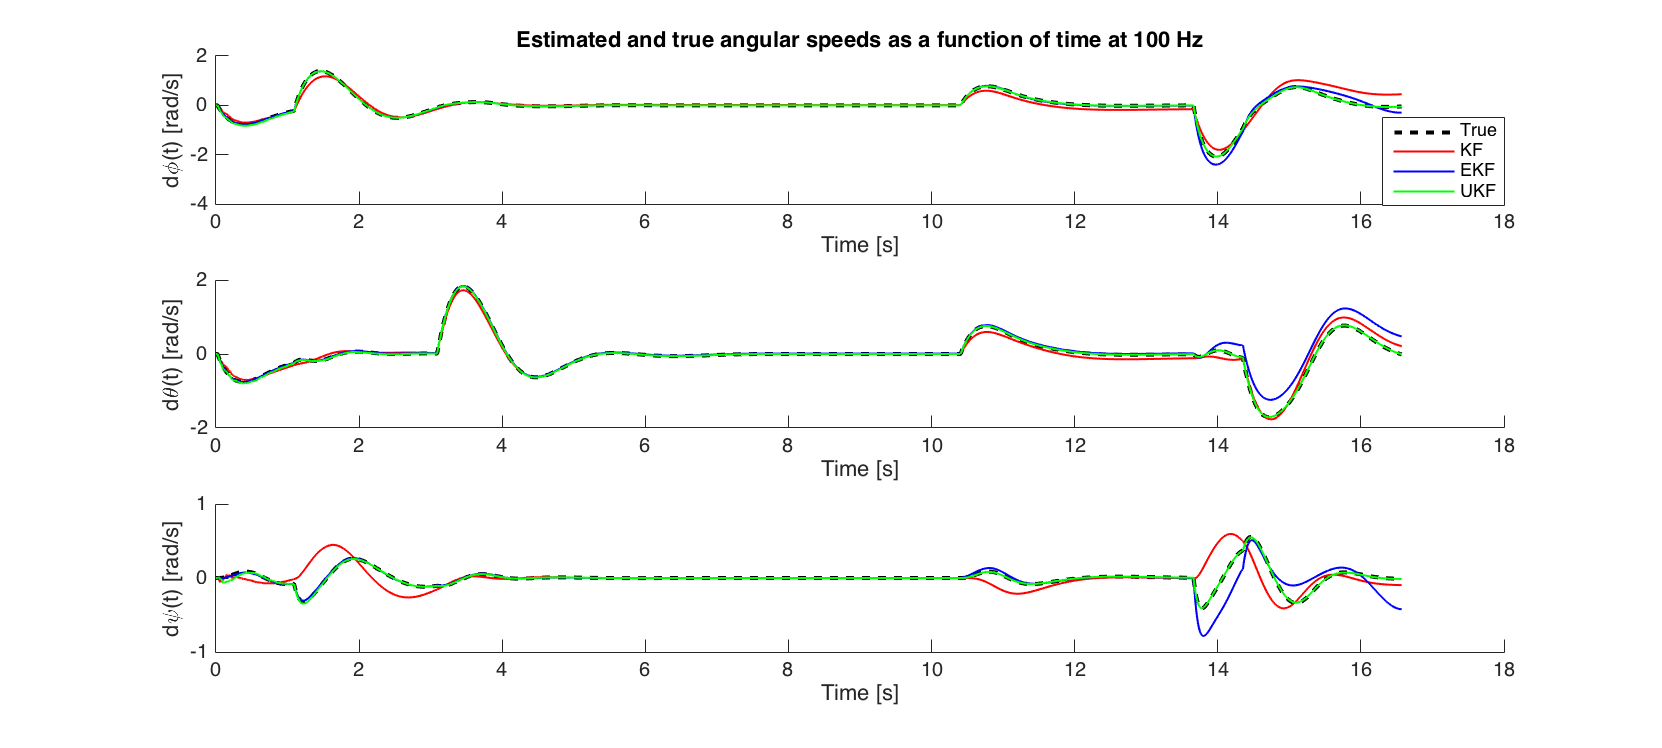
\includegraphics[width=1\textwidth]{figures/KalmanFilterComparison.png}
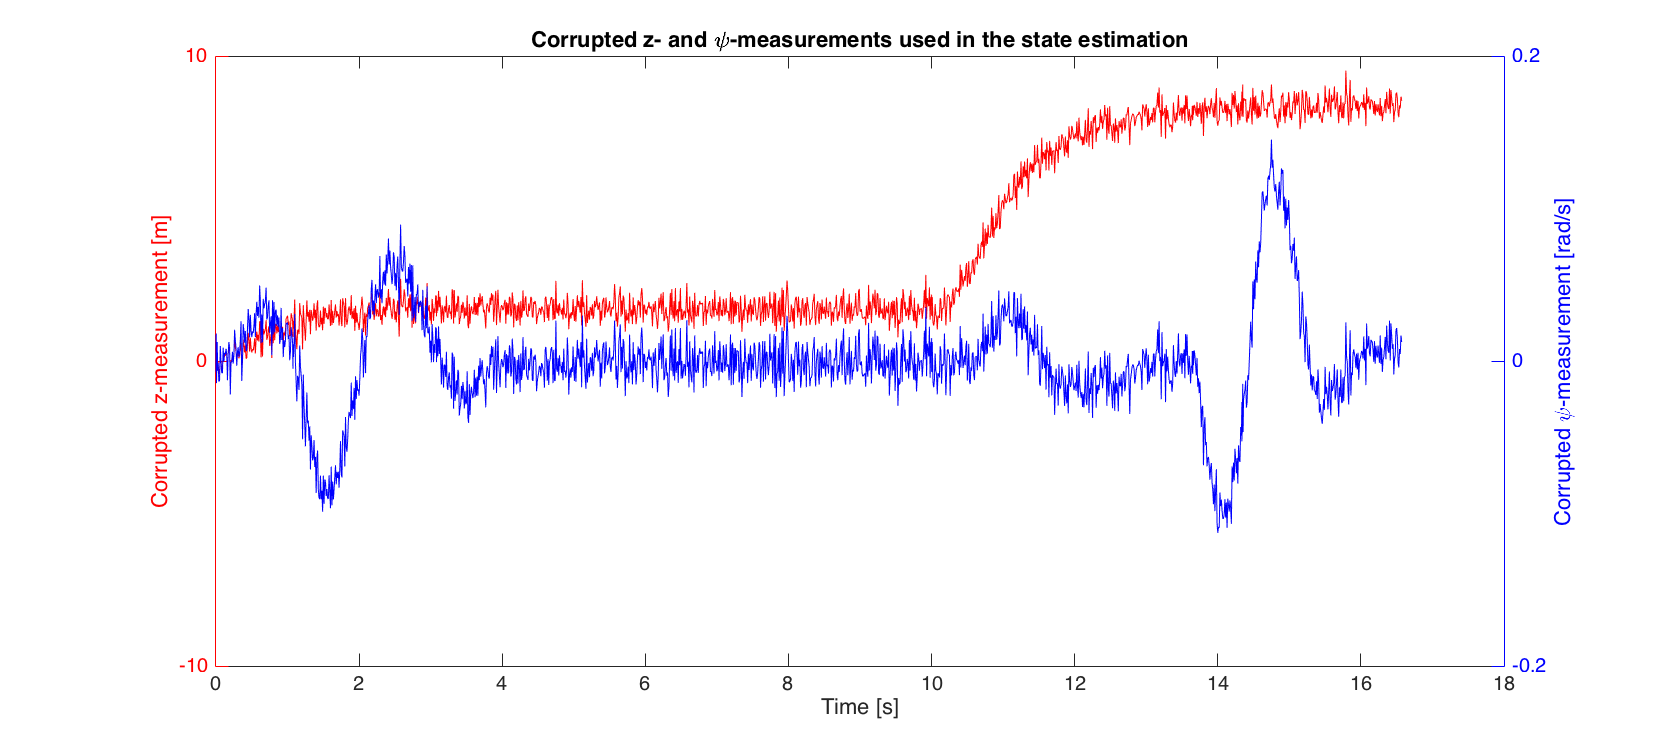
\includegraphics[width=1\textwidth]{figures/KalmanCompMeasurements.png}
\rule{35em}{0.5pt}
\caption{Demonstration of the drawbacks in using a regular Kalman compared to the EKF when estimating an unknown $\dot{\boldsymbol\eta}_k$, using (i) the same parameters in both filters (ii) having $\dot{\boldsymbol\eta}_k$ unknown and using (iii) corrupted measurements of $\boldsymbol\xi, \dot{\boldsymbol\xi}_k, \boldsymbol\eta_k$.}
\label{fig:KF-EKF}
\end{figure}

As can be seen, the regular KF performs badly when the system is far from the stable state, and the over all error is here visibly the largest. The EKF performs better, but when simulating the system at an inner loop sample rate of 100 Hz, the EKF is demands processing power to a point where it becomes infeasible to implement in the physical process (unless other methods of computing the Jacobian are considered). In addition, the EKF estimation becomes more unstable as the step size increases, and already at a sample period of $T_s = 0.01$ [s], the estimation becomes very poor after $\approx 16$ [s] and the covariance matrix requires resetting (at higher sample rates such as 500 Hz, the filter performs well for an entire simulation duration of 50 s). This is due to the approximations used in the covariance updates of the EKF, and it should be noted that the trajectory is very aggressive, and that the EKF may not diverge during the battery lifetime ($\approx5$ minutes) if following smother trajectories.

 The UKF has to be set with a fairly high $\alpha\approx0.5$ in order to spread the sigma points enough to properly capture the non-linear dynamics. It is far more economical in terms of computational power than the EKF and follows the true values much more accurately than any of the previously tested filters. This is clear when looking at the the error metric 
\begin{equation}\label{eq:errormetric}
E(\mathbf{x},\hat{\mathbf{x}}) = \sum^{3}_i\int_0^{t_s} |\dot{\boldsymbol{\eta}}_i(t) - \dot{\hat{\boldsymbol{\eta}}}_i(t)|dt
\end{equation}
for the the estimation of the unknown states during a simulation time $t_s = 17$ [s]. Here, $E_{KF} \approx 4.2768$, $E_{EKF} \approx2.4781$, $E_{UKF} \approx0.1990$ showing that for this specific problem, the UKF the the better alternative in terms of accuracy and computational power (compared to the EKF). In conclusion, the only viable option is to run the UKF in the inner loop, but the GPF has yet to be tested.

\subsubsection{Outer loop}
As we are using a linear model, the Kalman Filter will yield optimal estimations assuming the measurement noise is zero mean and gaussian. Consequently, the KF and an asynchronous variation of it was tested to cope with the delays when sending data to and from the crazyflie. To achieve this, two basic methods are considered. The first is to ignore the time delayed accelerometer data, and simply consider a 3-dimensional discrete time double integrator
\begin{equation}
\mathbf{x}_{k+1} =
\begin{bmatrix}
\mathbb{I} & h\cdot\mathbb{I}\\
\mathbf{0} & \mathbb{I}\\
\end{bmatrix}
{\mathbf{x}}_k
, \qquad \mathbf{y}_k = 
\begin{bmatrix}
\mathbb{I} & \mathbf{0}\\
\end{bmatrix}
{\mathbf{x}}_k
,\qquad \mathbf{0}, \mathbb{I}\in \mathbb{R}^{3\times 3}
\end{equation}
to filter the measured positions from the Kinect and estimate the velocities, with
\begin{equation}
\mathbf{x}_k = \begin{bmatrix} x & y & z  & \dot x & \dot y & \dot z  \end{bmatrix}^T.
\end{equation}
The second approach is to use discrete time triple-integrator model,
\begin{equation}
\mathbf{x}_{k+1} =
\begin{bmatrix}
\mathbb{I} & h\cdot\mathbb{I} & \frac{h^2}{2}\cdot\mathbb{I}\\
\mathbf{0} & \mathbb{I} & h\cdot\mathbb{I}\\
\mathbf{0} & \mathbf{0} & \mathbb{I}\\
\end{bmatrix}
{\mathbf{x}}_k
, \qquad \mathbf{y}_k = 
\begin{bmatrix}
\mathbb{I} & \mathbf{0} & \mathbf{0}\\
\mathbf{0} & \mathbf{0} & \mathbb{I} \\
\end{bmatrix}
{\mathbf{x}}_k
,\qquad \mathbf{0}, \mathbb{I}\in \mathbb{R}^{3\times 3}
\end{equation}
where
\begin{equation}
\mathbf{x}_k = \begin{bmatrix} x & y & z  & \dot x & \dot y & \dot z  & \ddot{x} & \ddot{y} & \ddot{z}  \end{bmatrix}^T.
\end{equation}

The KF and AKF are then applied to the measurements as seen on the host computer, i.e. the noisy positions (no delay) and, if applicable, vey noisy acceleration measurements delayed by some time $t_1\sim\mathcal{N}(0.03,0.002)$ [s], where the variance captures non-deterministic behaviour of the ROS publishers and subscribers. The estimated outputs of the filters are then delayed by $t_1$ again (to simulate being sent back to the crazyflie), and are then compared to the true values. As a simple test, a reasonably aggressive one dimensional acceleration and the corresponding position were used as ground truth values, and the filter was run at 30 Hz corresponds roughly to how fast data is generated by the kinect 1 camera. The estimated states were then moving average filtered (unweighted MA of order 10) which has a negligible phase lag at the frequencies of 0.4 Hz (see Figure~\ref{fig:KF-AKF}). Note that neither method is dependent of complete system dynamics, and won't require too much bandwidth in the communication between the host and the crazyflie.

\begin{figure}[htbp]
\centering
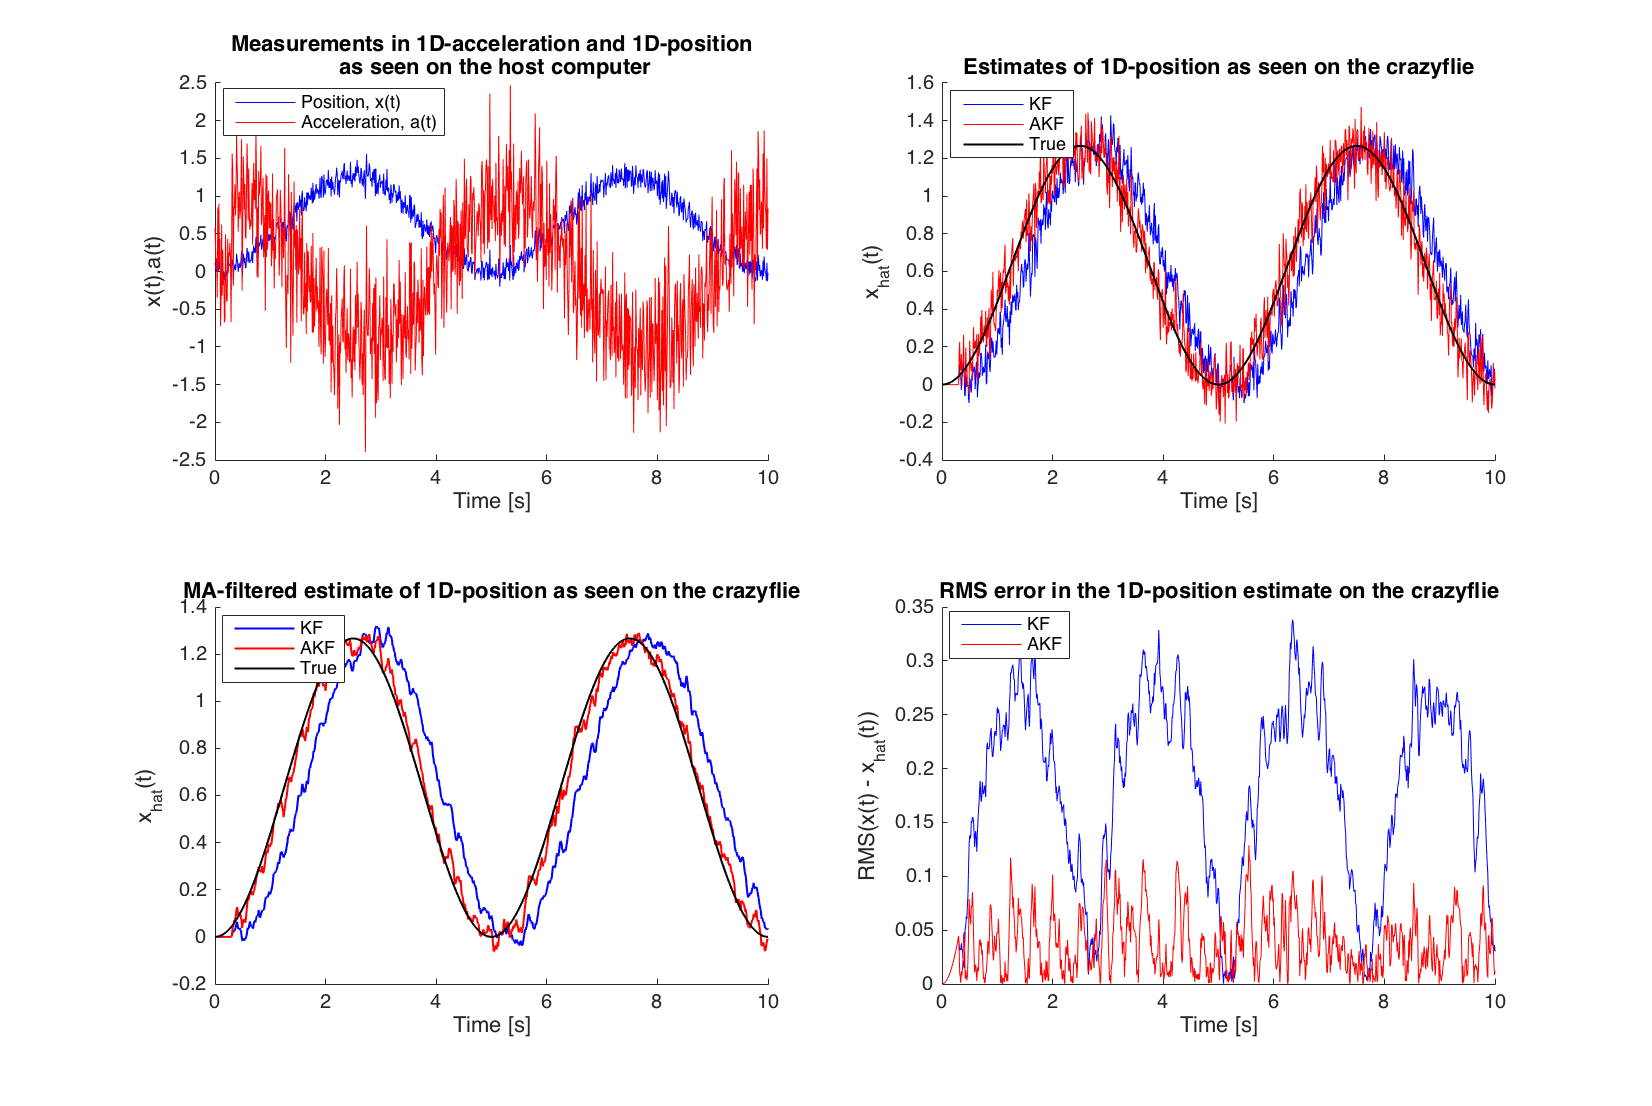
\includegraphics[width=1\textwidth]{figures/AKF-KFcomp.png}
\rule{35em}{0.5pt}
\caption{Comparison between KF and AKF using a 1D discrete triple integrator. \textit{Top left}: The measured acceleration and position as seen on the host computer, the true values have been heavily corrupted by noise and the acceleration is delayed by $t_1$. \textit{Top right}: The estimated positions using the KF and AKF as seen on the crazyflie compared to the true position. Here the positional estimates from the kalman filters have been delayed another $t_1$ before reaching the quadcopter. \textit{Bottom left}: The MA-filtered estimates (unweighted, order 10) as seen on the crazyflie compared to the true position (black). \textit{Bottom right}: The RMS error between the estimated position and true position when the data reaches the crazyflie with KF (blue) and AKF (red). }
\label{fig:KF-AKF}
\end{figure}


\section{Motion planning}\label{sec:reftraj}
In this part of the project, we consider the polynomial generation method advanced by Roy et.al. cite XX. The general method is presented to make the Matlab code coherent, using the same nomenclature as in the code, but the interested reader is referred to cite XX where the method is qualitatively compared with the Rapidly exploring Random Tree algorithms (RRT*) and a more numerically stable method is defined. The general idea is to set up a constrained QP problem and solve it (here using Matlab's \texttt{quadprog}) to find a minimum snap trajectory in space and time. The code will later be rewritten in Python/ROS with CVXGEN, and additional constraints will be enforced to ensure that the trajectory always stay in safe convex regions of space. These regions can conceivably be computed using the Iterative Regional Inflation by Semidefinite programming algorithm (IRIS) developed at MIT, but initially we assume assumed these regions to be known.

Let the trajectory be composed of $n$ polynomials $P_{1}(t),...,P_{n}(t)$, where
\begin{equation}
P_{k}(t) = \sum\limits_{i = 0}^N p_it^i, \qquad t\in[0,T_k]
\end{equation}
with a maximum degree of $\deg(P_{k})=N$, and a corresponding coefficient vector $\mathbf{p}_{(k)}=[p_{k,0},...,p_{k,N}]$. The problem is then to minimise a cost function for every polynomial spline
\begin{equation}
J(T_k) = \int_0^{T_k} c_0P_{k}(t)^2 +  c_1P^{\prime}_k(t)^2  + ... + c_NP^{(N)}_{k}(t)^2 dt = \mathbf{p}_{(k)}^T\mathbf{Q}_{(k)}\mathbf{p}_k
\end{equation}
such that continuity is preserved and boundary conditions are enforced. In cite XX, the hessian matrix corresponding to a polynomial was derived by differentiating the term in the cost function containing the $r^{th}$ derivative of $P_{(k)}(t)$ with regards to the polynomial coefficients $p_i$, i.e. finding
\begin{equation}
\mathbf{Q}_{r,(k)}= \frac{\partial^2}{\partial p_i\partial p_j} \int_0^{T_k} P_{k}^{(r)}(t)^2dt
\end{equation}
and constructing the matrix
\begin{equation}
\mathbf{Q}_{(k)}=\mathbf{Q}_{(k)} = \sum\limits_{r = 0}^N c_r\mathbf{Q}_{r,(k)}\in \mathbb{R}^{(N+1)\times (N+1)}
\end{equation}
The complete constrained QP-formulation, including all $n$ polynomials is then
\begin{equation}
\text{Minimize}\Big(\sum_{k=1}^nJ(T_k)\Big)\qquad\text{subject to}\qquad\mathbf{A}\mathbf{p}-\mathbf{b}=0
\end{equation}
where
\begin{equation}
\end{equation}
\begin{equation}
\sum_{k=1}^nJ(T_k) =
\begin{bmatrix}
\mathbf{p}_{(1)} & \cdots & \mathbf{p}_{(n)}
\end{bmatrix}
\begin{bmatrix}
\mathbf{Q}_{(1)} & 0 & 0 \\
0 & \ddots & 0 \\
0 & 0 & \mathbf{Q}_{(n)}
\end{bmatrix}
\begin{bmatrix}
\mathbf{p}_{(1)} \\ \vdots \\ \mathbf{p}_{(n)}
\end{bmatrix}
 = \mathbf{p}^T\mathbf{Q}\mathbf{p}.
\end{equation}
For the $k^{th}$ polynomial, the $r^{th}$ derivative can be written
\begin{equation}\label{eq:polyderiv}
P_k^{(r)}(t) = \sum_{n=r}^N\Big(\prod_{m=0}^{r-1}(n-m)\Big)p_{k,n}t^{n-r}.
\end{equation}
Using this formula, boundary conditions can be enforced for each spline by finding a matrix 
\begin{equation}
\mathbf{A}_{(k)}
\mathbf{p}_{(k)} = 
\mathbf{b}_{(k)}
\end{equation}
for every know derivative at the time $t=0$ (collected in $\mathbf{A}_0$) and time $t=T_k$ (collected in $\mathbf{A}_T$). With $n_c$ boundary conditions for the $k^{th}$ spline, then
\begin{equation}
\mathbf{A}_{(k)} = 
\begin{bmatrix}\mathbf{A}_{0,k}\\
\mathbf{A}_{T,k}
\end{bmatrix}\in\mathbb{R}^{n_c\times N+1}
\quad\text{and}\quad
\mathbf{b}_{(k)} = 
\begin{bmatrix}\mathbf{b}_{0,k}\\
\mathbf{b}_{T,k}
\end{bmatrix}\in\mathbb{R}^{n_c\times1}
\end{equation}
For the remaining, free boundary endpoints where no fixed derivative is specified, the splines on each side of a boundary point are set equal by enforcing
\begin{equation}\label{eq:cont}
\mathbf{A}_{T,k}\mathbf{p}_k - \mathbf{A}_{0,k+1}\mathbf{p}_{k+1}=0.
\end{equation}
A general method of generating the $\mathbf{Q}$- and $\mathbf{A}$-matrices was implemented in matlab (see \texttt{get\_Q}, \texttt{get\_A}), called by the \texttt{compute\_splines} method which used \texttt{quadprog}'s interior point method to find a solution given a set of points, times and a cost vector. This, and the demo script \texttt{splines\_2\_1D\_example.m} is located in the /crazy\_trajectory directory and is almost in a good state. The problem can be solved using various polynomial degrees and finds connecting splines, but the continuity conditions in free points~\label{eq:cont} is still not working properly (see Figure~\ref{fig:splines}). Clearly, the jerk squared is minimised and the the polynomial splines are continuos, but the derivatives are not. We have yet to figure out why.
\begin{figure}[htbp]
\centering
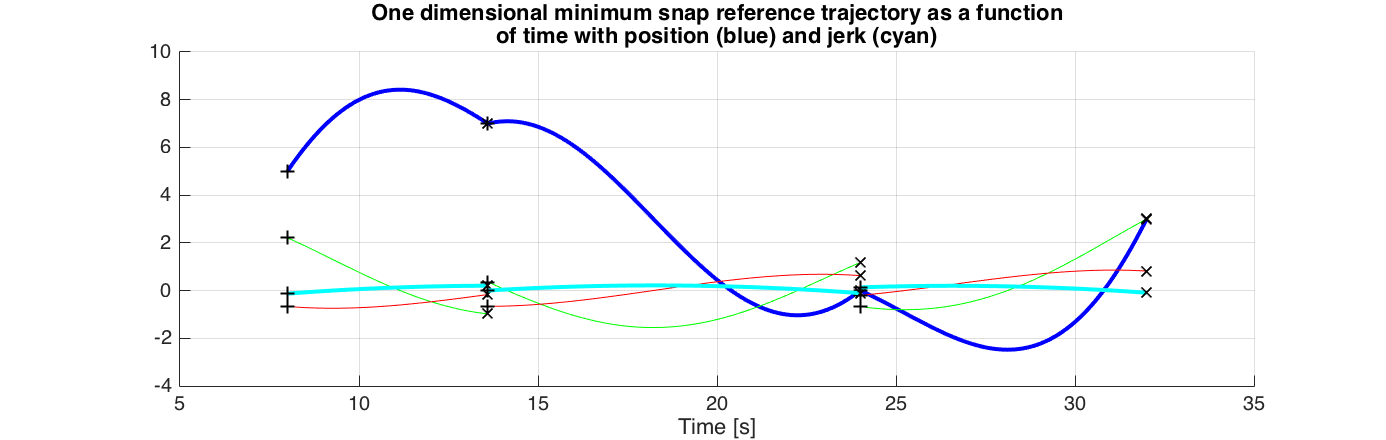
\includegraphics[width=0.8\textwidth]{figures/Splines.png}
\rule{35em}{0.5pt}
\caption{A reference trajectory composed of three splines with a maximum order of $N = 5$ and cost vector $c = [0,0,0,1,0,0]$ (minimum snap), enforcing positional endpoint conditions and at unevenly spaced times, with $t = [8,13.6,24,32]$.}
\label{fig:splines}
\end{figure}

\section{Outer control}
In this section, we wish to find a suitable outer controller to complement the stabilising inner controller. The main objectives is to utilise the computational power of the host computer to accurately follow trajectories in the $\mathbf{r}\dot{\mathbf{r}}$-space, as generated by the motion-planning QP-algorithm. For this purpose, a simple model independent PD controller was implemented as a reference, as a benchmark to measure performance of both model based MPC and $\mathcal{L}_1$-control. Here performance is evaluated in the error metric defined earlier~\eqref{eq:errormetric}, primarily with regards to positions and velocities in the global frame. The entire control system, complete with state estimation can then be viewed for the first time (see Figure~\ref{fig:controlsystem}).

\begin{figure}[htbp]
\centering
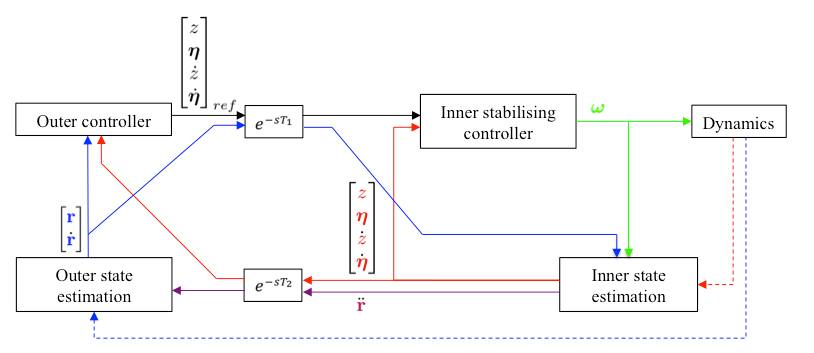
\includegraphics[width=0.8\textwidth]{figures/controlsystem.png}
\rule{35em}{0.5pt}
\caption{Overview of the entire system with system measurements of positions $\mathbf{r}$ from the kinect 1 (blue dashed) and measurements from the accelerometer, magnetometer, gyroscope and pressure sensor (red dashed).}
\label{fig:controlsystem}
\end{figure}

\subsection{PD-control}
The PD-controller is a very simple approach to  decent positional control. Here the yaw of the rotorcraft, $\psi$, is set to and assumed to be zero at all times, implying that increasing the pitch, $\phi$, while maintaining thrust to keep a desired elevation will move the quadcopter in the positive $x$-direction in the global coordinate system. Similarly, decreasing the roll, $\theta$, will move the quadcopter in the positive $y$-direction. As such, in this outer PD controller, we have a mapping
\begin{flalign}
\begin{split}
\phi_{ref}=&K_{D,x}({x}_{ref} - {x})) + K_{P,x}(x_{ref} - x)\\
\theta_{ref}=&K_{D,y}({y}-{y}_{ref})) + K_{P,y}(y-y_{ref} )
\end{split}
\end{flalign}
where the corresponding angular velocity references can be set to zero at all times for a more stable implementation, or as the numerical derivatives with a coefficient $N$ of the angular references. Note that in the former approach, no numerical derivatives are required in computing the control errors above, as the the trajectory is parametrised by polynomial splines in time, and can be derived analytically~\eqref{eq:polyderiv} in the reference generator.

This controller was implemented and tuned in Simulink, with $K_{P,\cdot}=0.2$ and $K_{D,\cdot}=0.17$. It was tested for the model parameters used in previous experiments, and the implementation was done by only computing the numerical derivatives of angular reference signals with $N=100$, thereby using the full potential of the trajectory planner.

\subsection{MPC}
For the MPC control, the system dynamics is augmented with stabilising PD control in \textbf{Section \ref{sec:PD}}, and linearised around a stable hovering point. The system was implemented in Matlab without state estimation using the MPC-tools 1.0 developed at LTH cite XX as a proof of concept (see \texttt{/Examples/quadcopter\_mpc\_position\_test.slx}). The result was equivalent to that of the PID-PD controller when using a fixed reference point for all states on the prediction horizon, and can be expected to improved if using time-varying reference generated in the motion planning. As the MPC-tools solution is (i) incredibly slow, (ii) unable to handle varying references on the prediction horizon and (iii) not apt for a Python/C-realtime implementation in ROS, alternatives were investigated. The two candidates are CVXgen and QPgen, which both generate fast QP solvers in C, and can be set up to suffice (i).

The MPC-problem formulation, with a time varying reference, $\mathbf{r}_k$, and a control signal, $\mathbf{u}_k$, kept close to the angular velocity required to hover, $\mathbf{u}^s$, can be written
\begin{flalign}
\begin{split}
\min\Big(\sum^{m}_{k=1}(\mathbf{x}_k - \mathbf{r} _k)^T\mathbf{Q}(\mathbf{x}_k - \mathbf{r} _k) + \sum^{n}_{k=1}(\mathbf{u}_k-\mathbf{u}^s)^T\mathbf{R}(\mathbf{u}_k-\mathbf{u}^s)\Big)\\
\mathbf{x}_{k + 1} = \mathbf{A}^d\mathbf{x}_k+ \mathbf{B}^d\mathbf{u}_k, \qquad k = 0,...,m\\
|\mathbf{x}_{7,k + 1}| < x_{max}, \qquad k = 1,...,m\\
|\mathbf{x}_{9,k + 1}| < x_{max}, \qquad k = 1,...,m\\
|\mathbf{u}_k - \mathbf{u}^s| < u_{max}, \qquad k = 1,...,n\\
||\mathbf{u}_{k} - \mathbf{u}_{k-1}||_{\infty} < S_{max}, \qquad k = 1,...,n\\
\end{split}.
\end{flalign}
Where $\mathbf{Q}\in\mathbb{R}^{10\times 10}_+, \mathbf{R}\in\mathbb{R}^{4\times 4}_+$ are diagonal cost matrices, $\mathbf{A}^d\in\mathbb{R}^{10\times 10}, \mathbf{B}^d\in\mathbb{R}^{10\times 4}$ are the ZOH-sampled, discrete time system matrices of the augmented state space model. The remaining constraints bound the pitch and yaw, bound the deviation in control signal from the linearisation point $\mathbf{u}^s$, and the final puts a hard constraint on how fast we allow the control signal to vary (slew rate). This final constraint can be set very high or removed completely, as the motors are incredibly responsive.

With this formulation with $m,n = 10$, the QP solver generated by CVXgen has 5364 non-zero KKT entries, which is slightly above the recommended 4000. To evaluate the feasibility of the CVXgen solver with the above formulation, a Simulink implementation was made using the MEX-solver, replacing the MPC-tools solver with a rewritten S-function (see \texttt{MPC\_CVX.m}). The solver seems to work perfectly with the simulink environment, and is, as suspected, incredibly much faster than the already implemented \texttt{qp\_is.m} solver of the MPC-tools. The implementation is still not complete, and can presently only be run as an open loop system, where $\mathbf{u}_0$ is set to 

In order to use The MPC solver efficiently, the reference trajectory generated by the optimisation in \textbf{Section \ref{sec:reftraj}} has to be evaluated on the prediction horizon, i.e, at each cycle of the MPC-loop, we need to find a matrix $\mathbf{R}_{ref} = \begin{bmatrix}\mathbf{r}_1 & \cdots & \mathbf{r}_m\end{bmatrix}$, which evaluates the splines. The splines are in an array of polynomial coefficients, $\mathbf{P}$, defined on $t\in[t_0,t_f]$. Numerical evaluation needs to be done $m$ times at a period time of $T_s$, starting at the current time, $t_c$. Special caution needs to be taken if a sample time $t_k \neq [t_0,t_f]$, in which case the quadcopter is set to hover in the appropriate end of the trajectory.

For these purposes, the scripts \texttt{reftraj\_compute\_example.m} and \texttt{reftraj\_eval\_example.m} were written. The former computes a trajectory in space with fixed positions at certain points in time, the derivatives are left free and currently, there is an issue with continuity, as described in \textbf{Section \ref{sec:reftraj}}. The latter forms the $\mathbf{R}_{ref}$-matrix, and the resulting reference samples on the prediction horizon is plotted (see Figure~\ref{fig:trajectory}).
\begin{figure}[htbp]
\centering
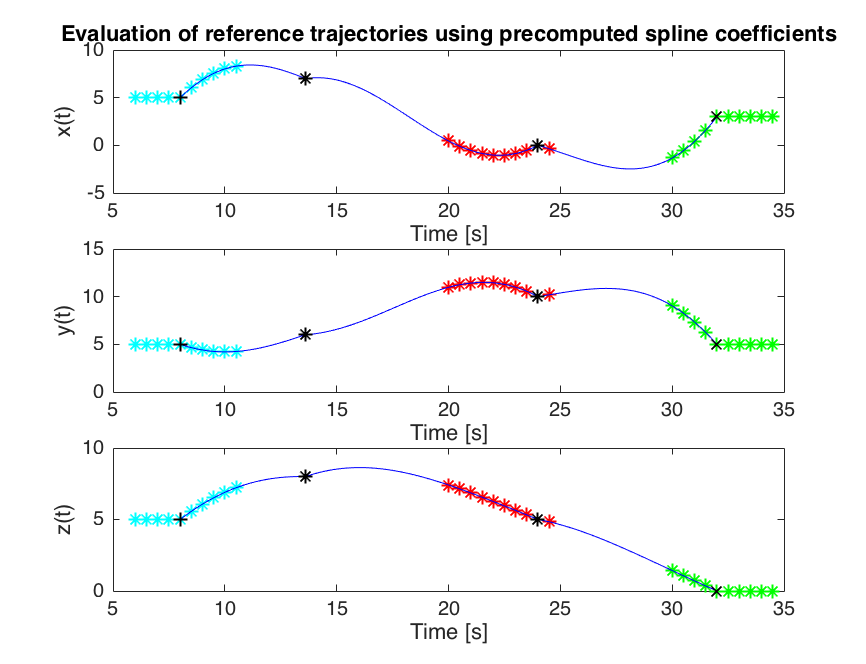
\includegraphics[width=0.5\textwidth]{figures/Trajectory.png}%
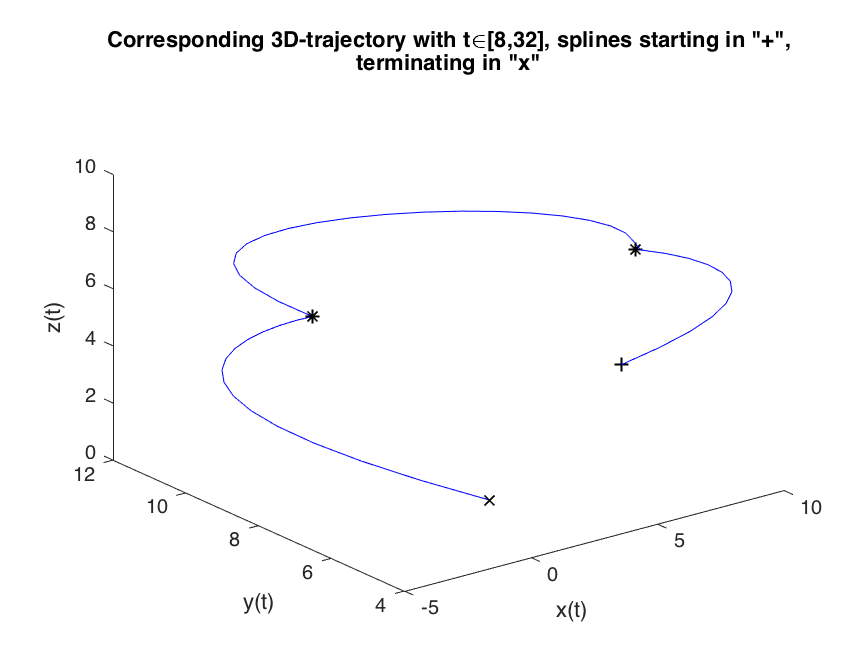
\includegraphics[width=0.5\textwidth]{figures/Trajectory3d.png}
\rule{35em}{0.5pt}
\caption{A reference trajectory composed of three 3D-splines with a maximum order of $N = 5$ and cost vector $c = [0,0,0,1,0,0]$ (minimum snap), enforcing positional endpoint conditions and at unevenly spaced times, with $t_0=8$ and $t_f=32$. The splines were evaluated with $T_s = 0.5$, $m = 10$, $t_c = 6\Rightarrow$ some $t_k < t_0$ (cyan), $t_c = 20\Rightarrow$ all $t_k\in[t_0,t_f]$ (red) and $t_c = 30\Rightarrow$ some $t_k > t_f$ (green). As can be seen, the algorithm properly evaluates the splines at evenly spaced times and makes the reference hover at a trajectory endpoint if $t_k\neq[t_0,t_f]$. Here, only the positional elements of $\mathbf{R}_{ref}$ are plotted, note the reference velocities and anles are also evaluated. }
\label{fig:trajectory}
\end{figure}

\subsubsection*{TODO}
\begin{enumerate}
\item \sout{Create simplified linearised system model for use in MPC} (see eg.~\cite{Bouffard:EECS-2012-241}).
\item \sout{Validate by comparison to the results in}~\cite{Bouffard:EECS-2012-241}.
\item \sout{Set up MPC controller with Simulink MPC-library} (see eg.~\cite{Bouffard:EECS-2012-241}).
\item \sout{Validate by comparison to the results in}~\cite{Bouffard:EECS-2012-241}.
\item Set up MPC controller with CVXgen and S-fucntions (see eg.~\cite{Bouffard:EECS-2012-241}~\cite{mattingley2012cvxgen}).
\item Validate by comparison to the results in Simulink.
\item System identification.
\item Simulate system with proper parameters.
\item Compare the four different implementations based on speed and stability.
\end{enumerate}

\subsection{$\mathcal{L}_1$-control}
The method of control formally known as $\mathcal{L}_1$-control has been highly debated since it's presentation in 2006~\cite{cao2006design}. Some claim it holds great promise and have proven it's effectiveness in various implementations, while others like Ortega and XX, claim it is not adaptive at all and that it can be reduced to a simple PI controller at all times. While both sides have strong arguments, we decided to implement and simulate $\mathcal{L}_1$-control of the quadcopter as it has already been done on a helicopter process with great success.

For the controller derivation, we consider control of the continuous time linearised system~\eqref{eq:linprocess}. The multidimensional $\mathbf{\Gamma}$-projection operator for two vectors $\theta,y\in\mathbb{R}^k$ is defined as
\begin{equation}
\text{Proj}_{\mathbf{\Gamma}}(\theta,y,f) =
\begin{cases}
\mathbf{\Gamma} y - \mathbf{\Gamma}\dfrac{\nabla f(\theta)(\nabla f(\theta))^T}{||\nabla f(\theta)||_2}\mathbf{\Gamma} yf(\theta)\qquad
\text{if}\;\;f(\theta)>0\;\;\text{and}\;\;y^T\nabla f(\theta)>0\\
\mathbf{\Gamma} y\qquad\qquad\qquad\qquad\qquad\qquad\quad\quad\text{otherwise}.
\end{cases}
\end{equation}
where $\mathbf{\Gamma} = \mathbb{I}_{k\times k}\Gamma$ for some scalar $\Gamma > 0$ (set as high as the CPU allows) and $f(\theta)$ is a convex function~\cite{L1control}~\cite{lavretsky2011projection}. By solving the Lyapunov equation
\begin{equation}
\mathbf{A}_m\mathbf{X}+ \mathbf{X}\mathbf{A}_m^T+ \mathbf{Q} = 0,
\end{equation}
for $\mathbf{P}=\mathbf{P}^T$, with some arbitrary $\mathbf{Q}>0$, the feedback controller
\begin{equation}
\begin{cases}
u(t)=\hat{\theta}^Tx(t)+k_gr(t)\\
\dot{\hat{\theta}}(t) = \text{Proj}_{\mathbf{\Gamma}}(\hat{\theta}^T(t),x(t)\tilde{x}^T(t)\mathbf{X}b)
\end{cases}
\end{equation}
can be constructed, where $\tilde{x} = \hat{x} - x$ is the state estimation error, $k_g$ is a gain and $r(t)$ is the reference signal. By designing the companion system
\begin{equation}
\begin{cases}
\dot{x}(t) = \mathbf{A}_m\hat{x}(t) + \mathbf{B}(u(t)-\hat{\theta}^T(t)x(t))\\
y(t) = \mathbf{C}^T\hat{x}(t)
\end{cases}
\end{equation}
it can be shown (by Theorem 2~\cite{cao2006design}) that the state estimation error,
\begin{equation}
\lim_{t\rightarrow\infty}\tilde{x} = 0.
\end{equation}
By a corollary of the theorem, choosing
\begin{equation}
k_g =-\frac{1}{\mathbf{C}^T\mathbf{A}_m^{-1}\mathbf{B}} \Rightarrow \lim_{t\rightarrow\infty}y(t) = r \quad \text{if}r \equiv \text{constant}. 
\end{equation}

We have successfully implemented our own projection operator an validated it against the example used by Cao in ~\cite{cao2006design}.Currently, the biggest difficulty is to define robustness metrics and perform the multi-objective optimisation to determine LP-filter coefficients satisfying the one-norm criterea~\cite{huynh20141}. Once this has been done, we should have fully operational $\mathcal{L}_1$-control.

\section{Real time implementation}
In the current commercial crazyflie software, communication with the crazyflie is facilitated by the BitCraze virtual machine (VM) in which the user can bootload and interact with the crazyflie using a PyQt-client and ZeroMQ. This is very convenient, as file structures and dependencies can be pre-installed in the VM, but there is great interest in migrating to a ROS based client, both by developers and users, to make the most of preexisting ROS-tools for visualisation and harder realtime control. Much work has been done by W. Hoenig to create a stable ROS driver for the crazyflie~\cite{HoenigMixedReality2015}. As such, communication between a host computer and the crazyflie has already been developed, but good methods of control and external state estimation have not yet been implemented. In this part of the project, we aspire to implement our own ROS structure from scratch, supporting external motion capture using kinect 1 cameras, communication with Hoenig's driver and shell-interaction with the entire ROS structure through a master node.

\subsection{General structure}
The realtime project revolves around a single module, the \texttt{crazylib.py} module located in /modules/. This module can be directly imported into the ROS nodes and currently supports discrete KF/AKF/UKF updates implemented as described in algorithms~\ref{fig:algKF}~\ref{fig:algAKF}~\ref{fig:algUKF}, as well as Cython wrappers for calling C-programs compiled as dynamical libraries, such as the CVXgen solver directly through the module. The workflow is to add necessary functions to the crazylib module, and then test them rigorously using the examples in the /modules/examples/ directory before finally including them in the ROS nodes.

The nodes are created from the files in the /scripts/ directory, where each node is described in a separate python file.  A node is a threading process which interacts with the roscore and through it other nodes over topics (using UDP/TCP). The data types sent between the nodes can be represented in various formats, and as we are using numpy for the most part, a set of custom message types were defined in the /msg/ directory. For example, the \texttt{NumpyArrayFloat64.msg} definition enables nodes to send ndarrays over the topics. The entire structure can be launched using the XML launch files in the /launch/ directory, which connects all of the Nodes in /scripts/ to the ROS master and also initialises openni (a driiver used to communicate with the kinect) and Hoenig's driver (used to communicate with the crazyflie).

All filter and model parameters are set in a JSON configuration file (.cnf) in the /config/ directory, which is then used to initialize all of the processes. This was created as a safety measure, so as not to set crucial parameters such as loop rates differently in different nodes. In addition, this makes it so that old configuration files can be stored, reused and compared in simulation without the need to set parameters in each node independently. So to summarise, the entire structure including nodes, lines of communication and configurations can all be launched by executing the single command
\begin{equation*}
\texttt{roslaunch crazy\_ros crazy.launch UseDummy:=0}
\end{equation*}

We structured the project so that, once launched, the master node initialises calibration of the kinect in the /kinectNode (see \textbf{Section}~\ref{sec:calibration}), which when complete allows the user to interact with the master directly in the terminal. Here the user can type \texttt{-h} for help, which then shows exactly which commands are possible and how the system is operated. For instance, commands can be sent to activate the PD controller, which then deactivates the MPC controller and referenceGenerator node, and vice versa. Executing the command \texttt{q} the system sets all control signals to 0 and halts completely as a safety measure. in addition, the control signals can either be sent to the crazyflie directly, or to the quadcopterModel, which then simulates the discrete time system using the crazylib module and publishes the states to the /measuredstates topic, where they can be visualised using \texttt{rqt\_plot}, \texttt{rviz} or simply stored recorded into bagfiles in the /bagfiles/ directory for postprocessing in Matlab.
\begin{figure}[htbp]
\centering
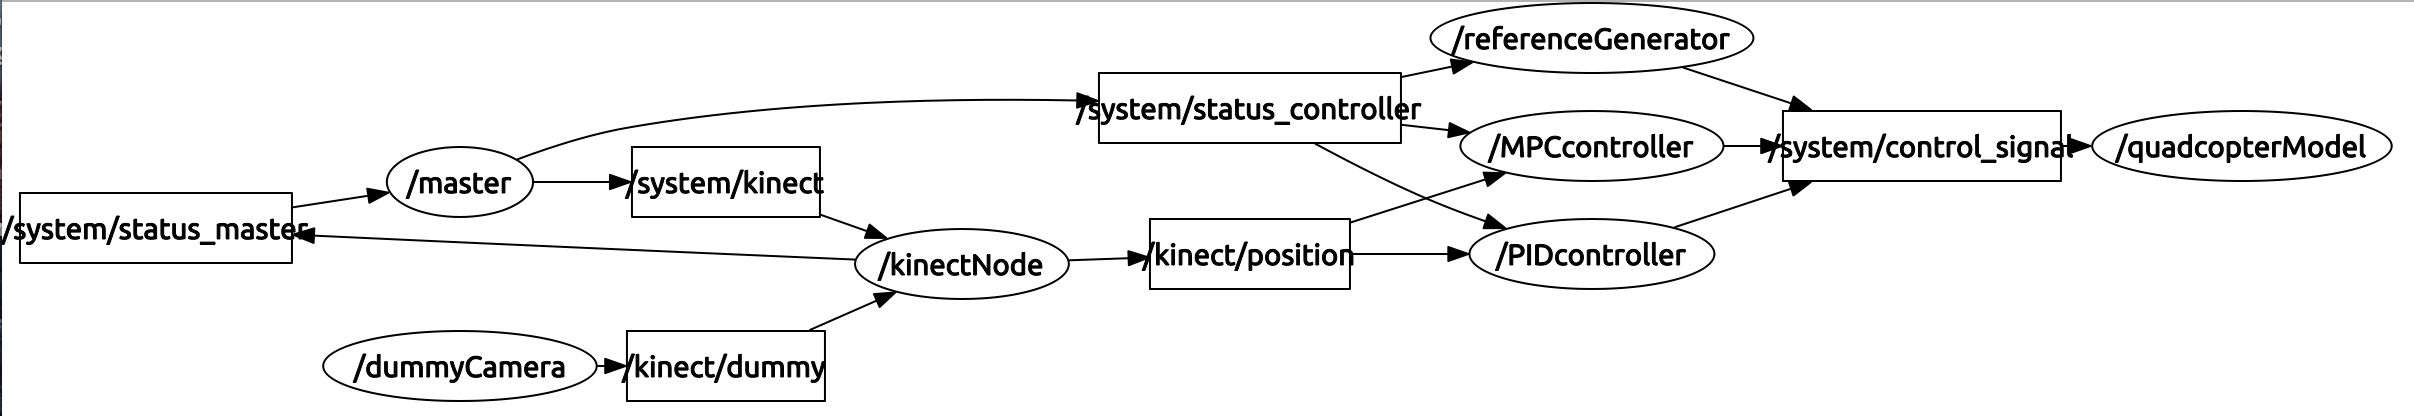
\includegraphics[width=\textwidth,trim={1mm 0 0 0.7mm},clip]{figures/ROSstruct.png}
\rule{35em}{0.5pt}
\caption{The current ROS structure as generated in \texttt{rqt\_plot} with nodes (ellipses), topics (boxes) and the connecting arrows intdicating the flow of information.}
\label{fig:ROSstruct}
\end{figure}
\subsection{Kinect node}
The kinect node subscribes to the /camera/depth/image\_rect-topic, to which the ``openni''-driver publishes information in the data type \texttt{Image}, which is part of the standard ROS messages library \texttt{sensor\_msgs}. This node handles the raw camera data and publishes the quadcopter position to the topic /kinect/position in the standard data type \texttt{Point} of the \texttt{geom\_msgs} library. The reason for this choice of data type is to enable real time plotting of the position. In this node the outer state estimation is done in order to minimise the non-deterministic effects of inter node communication via publishing/subscribing (recall UDP/TCP). Consequently, the purpose of the kinect node is to (i) calibrate the camera, (ii) handle and filter image data from the ``openni''-driver and (iii) facilitate communication between the kinect and the master. 

\subsubsection{Calibration}\label{sec:calibration}
The camera is calibrated by taking first taking 30 consecutive samples of the background noise, from which a mean depth is computed. When running, the measured depth matrix is subtracted with the background noise so that only a handful of pixels are zero separate (or rather above some threshold $\epsilon\approx 2$ depth units). This set of pixels, $S$, is then used to compute the depth of the copter as the mean of the depths of all pixels in $S$. Similarity, the quadcopter position in the image is computed as the mean of all x and y pixel indices of the points in $S$.

The angle of the camera is calibrated by taking a set of $N$ measurement points, $\mathbf{p}_i=\begin{bmatrix}x_i,y_i,z_i\end{bmatrix}$, in the background depth matrix. From these points, the center of mass is computed as
\begin{equation}
\bar{\mathbf{p}}= \begin{bmatrix}\bar{x},\bar{y},\bar{z}\end{bmatrix} = \frac{1}{N}\sum_{i = 1}^N \mathbf{p}_i,
\end{equation}
and a matrix for each point's deviation from the center of mass is set up
\begin{equation}
\mathbf{P} = \begin{bmatrix}\mathbf{p}_1\\ \vdots \\ \mathbf{p}_N\end{bmatrix} -  \begin{bmatrix}\bar{\mathbf{p}}\\ \vdots \\ \bar{\mathbf{p}}\end{bmatrix}\in\mathbb{R}^{N\times 3},
\end{equation}
The matrix $\mathbf{P}$ is then factorised using the singlar value decomposition (SVD), from which, the left-singular vector corresponding to the smallest of the three singular values is the normal of the best fitting plane in a least-squares sense, $\bar{\mathbf{n}}_{xyz}$. As we are only interested in the angle $\alpha$ in the $xz$-plane, the normal is projected onto this plane, resulting in the normal $\bar{\mathbf{n}}_{xz}$ (see Figure~\ref{fig:planecalibration}). From this, the angle is simply computed using the cosine dot product definition
\begin{equation}
\alpha = \arccos\Big(\frac{\bar{\mathbf{n}}_{xz}\cdot \hat{\mathbf{x}}_c}{||\bar{\mathbf{n}}_{xz}||_2}\Big).
\end{equation}

\begin{figure}[htbp]
\centering
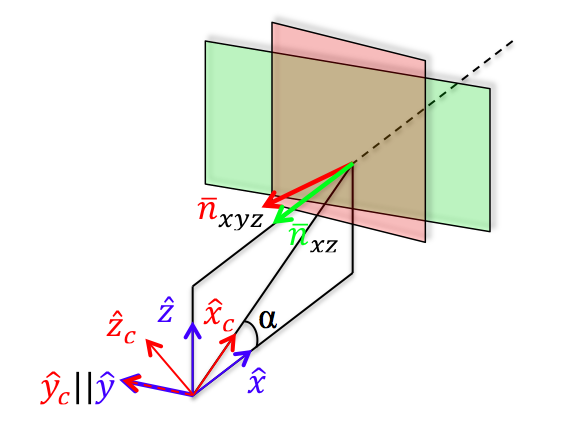
\includegraphics[width=0.5\textwidth]{figures/kinectcal.png}
\rule{35em}{0.5pt}
\caption{An illustration of SVD-calibration with the global coordinate system (blue), the camera coordinate system (red), the real life wall defined in three dimensions (red) and the projected wall defined in two dimensions (green).}
\label{fig:planecalibration}
\end{figure}

Once the angle has been computed, we are ready to detect moving objects. By subtracting the background data from each measured image and computing the center of mass of all the points in $S$, we get an estimate of the quadcopter's center of mass in terms of depth and pixel indices. This point is then mapped into the camera coordinate system [m], where the depth unit is mapped to a distance from the camera to the quadcopter [m]  is used to translate the position of the copter to a point in space in the camera coordinate system, $\mathbf{p}_c$, with origin at the camera. This point is then translated into the global coordinate system, $\mathbf{p}$, (in which the controller operates) by means of the transformation
\begin{equation}
\mathbf{p} = \begin{bmatrix} \cos(\alpha)& 0 & -\sin(\alpha) \\ 0 & 1 & 0 \\ \sin(\alpha) & 0 & \cos(\alpha)\end{bmatrix} \mathbf{p}_c.
\end{equation}

\subsubsection{Filtering}
Once a positional measurement has been established in the global coordinate system, a Kalman filter is applied to smooth out the measurement and estimate the velocities of the quadcopter. The kalman filters were implemented in the \texttt{crazylib} module in the /crazy\_ros/modules/ directory, from which the discrete kalman update is called to update the estimation and covariance matrix for every new measurement. A big problem in the estimation is the cases when the copter is temporarily lost in the frame (which occurs frequently when flying $\sim$2 [m] from the camera). This problem was amended in practice by putting a small paper box on the bottom of the quadcopter, but also in the code by only using the complete kalman update when a good measurement is registered. In terms of software, two approaches were considered; (1) setting the measurement covariance matrix very high for bad measurements (rendering the kalman gain very small) and (2) by simply terminating the kalman update after prediction when a bad measurement is registered. In ROS, the second alternative is implemented, and the criteria for a bad measurement is defined by comparing the difference of the previous estimation and the current measurement (in the two-norm) and comparing this to the variance of the positions. By setting the initial covariance as a diagonal matrix (or toeplitz) with a main diagonal  $\geq1$, formulating the condition this way will allow higher two-norm deviations when beginning the filtering (which is desired, as the initial condition will never be perfect). The condition for a bad measurement on the $k^{th}$ update can then be written 
\begin{equation}
||\begin{bmatrix}\hat{x}^{k-1},\hat{y}^{k-1},\hat{z}^{k-1}\end{bmatrix}^T - \begin{bmatrix}x^k,y^k,z^k\end{bmatrix}^T||_2 < \alpha||\begin{bmatrix}\mathbf{P}_{11}^{k-1},\mathbf{P}_{22}^{k-1},\mathbf{P}_{33}^{k-1}\end{bmatrix}||_2
\end{equation}

As a proof of concept, and to illustrate how the filter handles some of the problems, a regular Kalman filter was used on the 3D-double integrator model (not using quadcopter accelerometer data) when simply swinging the quadcopter in a thin line. In the experiment, $\alpha = 5$, $\mathbf{Q} =0.1\cdot\mathbb{I}\in\mathbb{R}^{6\times 6}$, $\mathbf{R} =5\cdot\mathbb{I}\in\mathbb{R}^{3\times 3}$, and the quadcopter is swung in the \textit{xz}-plane during $\approx 30 s$. The data was saved from the topics (as published in ROS) and then analysed and plotted offline in Matlab (see Figure~\ref{fig:KFROS}).
\begin{figure}[htbp]
\centering
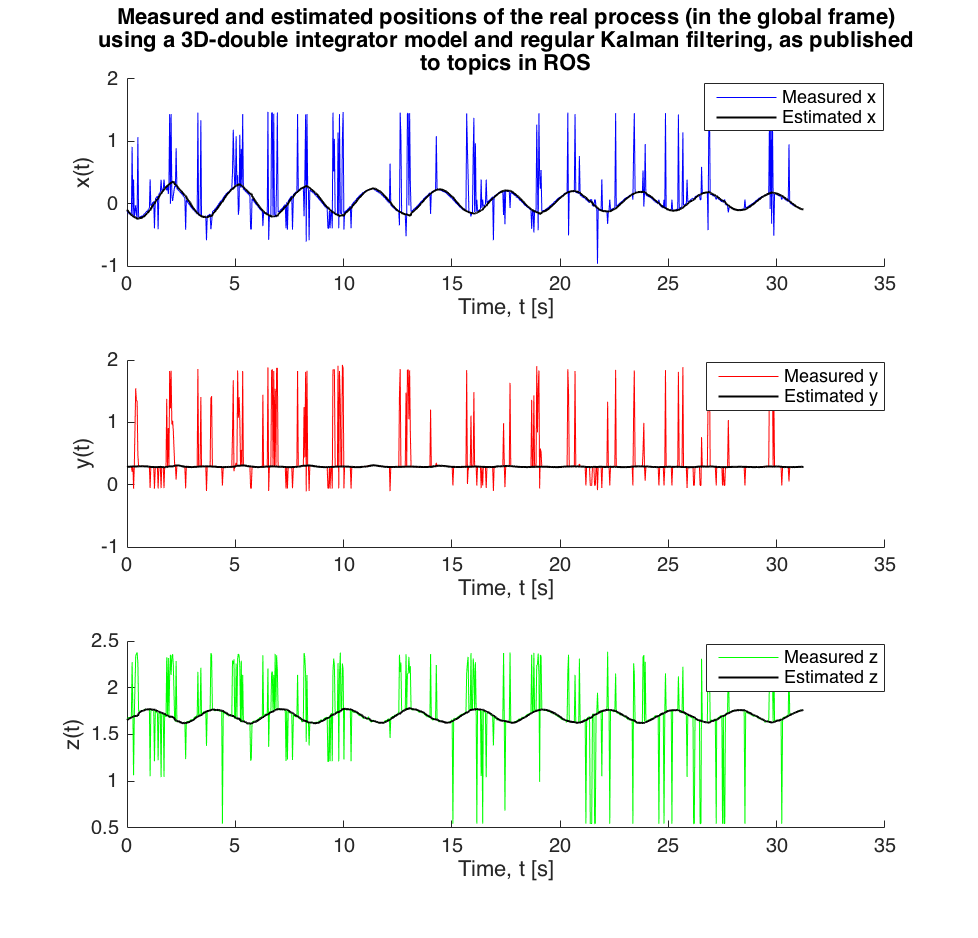
\includegraphics[width=0.7\textwidth]{figures/ROS_Kalman.png}
\rule{35em}{0.5pt}
\caption{.}
\label{fig:KFROS}
\end{figure}
Here we note that the filter handles outlying measurements very well (see the spikes in the measurement signals) and that the estimated positions are smooth and on a decaying harmonic oscillating form, as expected when the entire system then resembles that of a common pendulum. At no point is the quadcopter completely lost, and the result is good enough to continue with the real time PD/MPC implementations. 

\section{Summary}
The project has come a long way and many milestones have been met, but it has has been greatly slowed down by final exams and master thesis work. With that said, the work doesn't en here but will continue throughout the summer.
\subsection{Achieved goals and milestones}\label{sec:goalsandmilestones}
\begin{enumerate}
\item Successfully implemented a discrete version of the continuous dynamics derived by Lukkonen (\textit{Python/Simulink}).
\item Implemented and tuned a commonly used stabilising PD controller, tested LQG and implemented a novel tracking LQRi-controller with anti windup for the quadcopter platform, slightly outperforming previous methods of stabilisation (\textit{Simulink})
\item Created a state filtering S-fucntion toolbox in Simulink, supporting KF estimation for linear systems and EKF/UKF/AKF/GPF state estimation for non-linear systems complete with discrete double integrator examples (\textit{Simulink}).
\item Wrote and tested the crazylib module complete with methods for stat estimation (\textit{Python/ROS}).
\item Fixed errors in the MPC-tools 1.0 S-functions making the solver faster (\textit{Simulink}).
\item Functional positional MPC/PID control in (\textit{Simulink with MPCtools}).
\item Created Matlab based algorithms for finding the polynomial coefficients of a minimum snap trajectory 
\item Implemented operational ROS structure which ties together the Openni driver and Huning's ROS drivers and offers safe ways of interacting with the program and logging the data.
\item Developed new ways of calibrating the kinect 
\end{enumerate}

\newpage\bibliography{bibliography}{}
\bibliographystyle{IEEEtran}

\section{Appendix}\label{sec:appendix}
\end{document}